\chapter{Bound States in One Dimension}\label{ch:bound-states}

\begin{chapterintro}
A guitar string clamped at both ends can vibrate only in a discrete set of patterns: the fundamental, the second harmonic, the third, and so on. You met this in first-year physics, and you met its mathematical skeleton in Chapter~\ref{ch:eigen}, where the equation $-y''=\lambda y$ with fixed ends had eigenvalues $(k\pi/2L)^2$. A quantum particle trapped in a well behaves the same way. Its wavefunction must fit inside the well, and only special energies allow that. These special energies are the \emph{bound-state energies}, and the list of them is the particle's \emph{spectrum}.

In this chapter we solve the two exactly solvable wells that every physicist knows, the infinite square well (the ``box'') and the harmonic oscillator. We prove general facts that hold for every one-dimensional well: the energies are never degenerate, an even well has states that are alternately even and odd, and the $n$-th state has $n-1$ nodes. Then we ask the question that matters most for this book: how does the \emph{shape} of a well control the \emph{spacing} of its levels? We find a simple and physical answer: the level density equals the classical period divided by $2\pi$, so a well that widens quickly with energy, that is a potential that grows slowly, makes its levels crowd together.

Where this shows up in the paper: the paper's Hamiltonian $H=-d^2/dx^2+V(x)$ lives in a box $[-L,L]$ with Dirichlet walls (Sec.~II~B of \cite{soniR1}); its potential, the Wu--Sprung potential of Eq.~(2), is even; its levels are labeled from $n=1$ and the first 500 are scored at scale 1; and the slowly rising level density of the Riemann zeros is exactly what forces that potential to grow a little more slowly than a harmonic well. The parity facts of this chapter also explain why the paper's ``PT-odd'' perturbations have vanishing diagonal matrix elements (Sec.~II~E).
\end{chapterintro}

\begin{prerequisites}
\item Chapter~\ref{ch:schrodinger}: the time-independent Schr\"odinger equation $H\psi=E\psi$; the Born rule ($|\psi|^2$ is a probability density); normalization; Hermitian operators have real eigenvalues; the units $\hbar=2m=1$, in which $H=-d^2/dx^2+V(x)$.
\item Chapter~\ref{ch:eigen}: eigenvalues and eigenvectors; eigenvectors of a symmetric (Hermitian) matrix belonging to different eigenvalues are orthogonal; the string with fixed ends $-y''=\lambda y$; the second-derivative operator as a tridiagonal matrix; \texttt{scipy.linalg.eigh\_tridiagonal} as a black-box eigensolver.
\item Chapter~\ref{ch:fourier-series}: orthogonality of sines and cosines; even and odd functions.
\item Chapter~\ref{ch:complex}: complex conjugate.
\item First-year physics: potential-energy curves, turning points, simple harmonic motion (its period does not depend on amplitude), standing waves on a string.
\end{prerequisites}

%==========================================================
\section{What is a bound state?}\label{sec:bound-states-what}

\subsection{The classical picture}

Think of a marble rolling inside a bowl. If its total energy $E$ is less than the height of the bowl's rim, the marble rolls back and forth forever between two \emph{turning points} $x_1$ and $x_2$, where its potential energy $V(x)$ equals $E$ and its kinetic energy is zero. Between the turning points $E>V(x)$; this is the \emph{classically allowed region}. Outside them $E<V(x)$, which would require negative kinetic energy; this is the \emph{classically forbidden region}. A classical particle that stays forever in a bounded region is said to be \emph{bound}.

Classically, any energy above the bottom of the bowl is possible. Quantum mechanically, as we will now see, only special energies are.

\subsection{The quantum equation and the curvature rule}

Recall from Chapter~\ref{ch:schrodinger} that in units with $\hbar=2m=1$ the time-independent Schr\"odinger equation for a particle on a line is
\begin{equation}
-\psi''(x)+V(x)\,\psi(x)=E\,\psi(x),
\label{eq:bound-states-tise}
\end{equation}
where $\psi(x)$ is the wavefunction, $\psi''=d^2\psi/dx^2$, $V(x)$ is the potential energy and $E$ is the energy. The Born rule says $|\psi(x)|^2\,\dd x$ is the probability of finding the particle between $x$ and $x+\dd x$, so a physical state must be \emph{normalizable}:
\begin{equation}
\int |\psi(x)|^2\,\dd x = 1 ,
\label{eq:bound-states-norm}
\end{equation}
the integral running over the whole region available to the particle.

\begin{sample}{Real wavefunctions are enough}
Show that if $\psi$ solves \cref{eq:bound-states-tise} with real $V$ and real $E$, then so do its real part and its imaginary part.

\textbf{Step 1:} Take the complex conjugate of \cref{eq:bound-states-tise}. Since $V$ and $E$ are real (recall from Chapter~\ref{ch:schrodinger} that the eigenvalues of the Hermitian operator $H$ are real), conjugation acts only on $\psi$: $-(\psi^*)''+V\psi^*=E\psi^*$. So $\psi^*$ is a solution.

\textbf{Step 2:} The equation is linear: a sum of solutions with the same $E$ is a solution, and so is a constant multiple of one. Hence $\Re\psi=(\psi+\psi^*)/2$ and $\Im\psi=(\psi-\psi^*)/(2i)$ are solutions.

\textbf{Step 3:} At least one of them is not identically zero (otherwise $\psi=0$).

\[
\boxed{\text{For bound states we may always choose } \psi \text{ real.}}
\]
From now on all bound-state wavefunctions in this chapter are taken real, so $|\psi|^2=\psi^2$.
\end{sample}

Rewrite \cref{eq:bound-states-tise} as
\begin{equation}
\psi''(x)=\bigl[V(x)-E\bigr]\,\psi(x).
\label{eq:bound-states-curv}
\end{equation}
The second derivative is the \emph{curvature} of the graph of $\psi$. \Cref{eq:bound-states-curv} is a rule for the shape of the wavefunction:
\begin{itemize}
\item In an allowed region ($E>V$) the bracket is negative, so $\psi''$ has the sign opposite to $\psi$. Where $\psi>0$ the graph bends down, where $\psi<0$ it bends up: it always curves back toward the axis. The wavefunction \emph{oscillates}. If $E-V=k^2$ is constant, the solutions are $\cos kx$ and $\sin kx$; for example $(\cos kx)''=-k^2\cos kx$.
\item In a forbidden region ($E<V$) the bracket is positive, so $\psi''$ has the same sign as $\psi$: the graph curves away from the axis. If $V-E=\kappa^2$ is constant, the solutions are $e^{\kappa x}$ and $e^{-\kappa x}$; for example $(e^{-\kappa x})''=\kappa^2 e^{-\kappa x}$. A generic solution is a mixture of a growing and a decaying exponential.
\end{itemize}

\subsection{Why only special energies work: shooting}

Take the bowl-shaped potential $V(x)=x^2$, which is even, and look for an even solution. An even function has $\psi'(0)=0$ (its slope at the origin is zero), so start at $x=0$ with $\psi(0)=1$, $\psi'(0)=0$ and integrate \cref{eq:bound-states-curv} outward, like firing a projectile and watching where it lands. This is called \emph{shooting}. For $x$ beyond the turning point $\sqrt E$ the region is forbidden and the solution is some mixture of a growing and a decaying piece. For almost every $E$ the growing piece is present, and $\psi$ runs off to $+\infty$ or $-\infty$; such a $\psi$ violates \cref{eq:bound-states-norm}. \Cref{fig:bound-states-shooting} shows what happens: for $E=0.9$ the solution has not curved enough and shoots up; for $E=1.1$ it has curved too much and shoots down. Between them, at exactly $E=1$, it decays to zero.

\begin{figure}[htbp]\centering
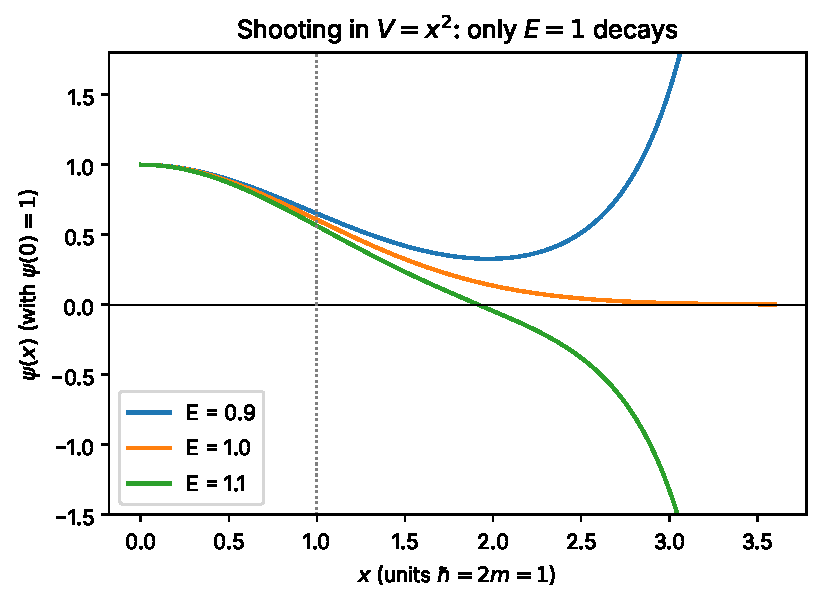
\includegraphics[width=0.85\linewidth]{figs/bound-states_shooting.pdf}
\caption{Shooting in the potential $V=x^2$ (units $\hbar=2m=1$). Each curve solves $\psi''=(x^2-E)\psi$ with $\psi(0)=1$, $\psi'(0)=0$. For $E=0.9$ the solution diverges upward, for $E=1.1$ downward; only at $E=1$ does it decay, giving a normalizable (bound) state. The dotted vertical line is the classical turning point $x=1$ of the $E=1$ state.}
\label{fig:bound-states-shooting}
\end{figure}

There is a counting argument behind this picture. A second-order equation has two independent solutions. Decay at the right end is one condition, and decay at the left end is another. The overall size of $\psi$ is free (it is fixed afterward by normalization), so only one combination of the two solutions is at our disposal, and it cannot generally meet two conditions. The energy $E$ is the extra knob that must be tuned. This is a heuristic; the rigorous statement is in the box below.

\begin{beyond}
\textbf{Taken on trust: discreteness of the spectrum.} Call a potential \emph{confining} if $V(x)\to+\infty$ as $|x|\to\infty$, or if the particle is confined to a finite interval by walls. For a confining potential that is continuous (or has finitely many jumps) inside the region, the normalizable solutions of \cref{eq:bound-states-tise} exist only for a discrete sequence of real energies $E_1<E_2<E_3<\cdots$ with $E_n\to\infty$, and the corresponding eigenfunctions form a complete orthonormal set. The proof belongs to Sturm--Liouville theory; see \cite{rhb} for the theory of such eigenvalue problems and \cite{griffiths} for the physics. The finite-difference version of this statement (Chapter~\ref{ch:eigen}) is the fact that a symmetric $N\times N$ matrix has $N$ real eigenvalues with orthogonal eigenvectors.
\end{beyond}

A normalizable solution of \cref{eq:bound-states-tise} is called a \emph{bound state}. In this book, as in the paper, we label the bound states in order of increasing energy starting from $n=1$: $E_1$ is the \emph{ground state}, $E_2$ the first excited state, and so on.

\subsection{The energy is always above the bottom of the well}

\begin{sample}{A lower bound on every bound-state energy}
Let $V_{\min}$ be the smallest value of $V$ on the region. Show that every bound state has $E>V_{\min}$. Assume, as holds for bound states, that $\psi\psi'\to 0$ at the ends of the region (at walls $\psi=0$; at infinity both $\psi$ and $\psi'$ tend to zero).

\textbf{Step 1:} Multiply \cref{eq:bound-states-tise} by the real, normalized $\psi$:
\[ -\psi\psi''+V\psi^2=E\psi^2. \]

\textbf{Step 2:} Integrate over the region $a<x<b$ and use \cref{eq:bound-states-norm}:
\[ -\int_a^b\psi\psi''\,\dd x+\int_a^b V\psi^2\,\dd x=E. \]

\textbf{Step 3:} Integrate the first term by parts with $u=\psi$, $\dd v=\psi''\,\dd x$:
\[ -\int_a^b\psi\psi''\,\dd x=-\bigl[\psi\psi'\bigr]_a^b+\int_a^b(\psi')^2\,\dd x=\int_a^b(\psi')^2\,\dd x \quad\text{(boundary term zero)}. \]

\textbf{Step 4:} Therefore
\begin{equation}
E=\int_a^b(\psi')^2\,\dd x+\int_a^b V\psi^2\,\dd x .
\label{eq:bound-states-energy-split}
\end{equation}
The first integral is the expectation value of the kinetic energy; the second is the expectation value $\langle V\rangle$.

\textbf{Step 5:} Since $V\ge V_{\min}$ everywhere and $\psi^2\ge0$, $\int V\psi^2\,\dd x\ge V_{\min}\int\psi^2\,\dd x=V_{\min}$.

\textbf{Step 6:} $\int(\psi')^2\,\dd x\ge 0$, with equality only if $\psi'=0$ everywhere, that is $\psi$ constant. A constant that vanishes at the ends (or at infinity) is zero, which is not normalizable. So the first integral is strictly positive.

\[ \boxed{E>V_{\min}} \]
\end{sample}

This is the quantum version of ``the marble cannot sit still at the bottom'': confinement always costs kinetic energy. The lowest energy $E_1$ minus $V_{\min}$ is called the \emph{zero-point energy}.

\begin{checkpoint}
The paper's Wu--Sprung potential has its minimum $V_0=3.10073\pi\approx 9.741$ at $x=0$ (Sec.~II~B of \cite{soniR1}). Is it consistent that its lowest level should approximate the first zeta zero $t_1=14.134725$?
\end{checkpoint}
\checkanswer{Yes. Every bound-state energy must exceed $V_{\min}=9.741$, and $14.13>9.741$. A lowest level below $9.741$ would be impossible for any potential with this minimum.}

\begin{keyideas}
\item A bound state is a normalizable solution of $-\psi''+V\psi=E\psi$; for real $V$ it can be chosen real.
\item Curvature rule: $\psi''=(V-E)\psi$. Allowed regions ($E>V$): oscillation. Forbidden regions ($E<V$): exponential growth or decay.
\item Only special energies give decay on both sides; for a confining potential they form a discrete list $E_1<E_2<\cdots$ (theorem taken on trust).
\item $E=\int(\psi')^2\dd x+\int V\psi^2\dd x$, so every level lies strictly above the bottom of the well.
\end{keyideas}

%==========================================================
\section{The infinite square well}\label{sec:bound-states-box}

\subsection{Setting up the box}

The simplest well is a region of zero potential with impenetrable walls:
\begin{equation}
V(x)=\begin{cases}0, & -L<x<L,\\ +\infty, & |x|\ge L,\end{cases}
\label{eq:bound-states-boxV}
\end{equation}
where $L$ is the \emph{half-width} of the box. (We center the box at the origin because the paper does: its domain is $[-L,L]$.) The particle cannot be in the walls, so $\psi=0$ there. Physically, you can picture the infinite wall as the limit of a very high finite wall: inside a wall of height $V_w$ the wavefunction decays like $e^{-\kappa|x|}$ with $\kappa=\sqrt{V_w-E}$, and as $V_w\to\infty$ the decay becomes instantaneous. We adopt as the definition of the infinite well that $\psi$ is continuous and vanishes at the walls:
\begin{equation}
\psi(-L)=0,\qquad \psi(L)=0.
\label{eq:bound-states-dirichlet}
\end{equation}
Conditions that fix the value of $\psi$ at the boundary are called \emph{Dirichlet} boundary conditions, and the walls are called Dirichlet walls. (The derivative $\psi'$ jumps at an infinite wall; only $\psi$ itself is required to be continuous there.)

Inside the box, \cref{eq:bound-states-tise} reads
\begin{equation}
-\psi''=E\psi,\qquad -L<x<L.
\label{eq:bound-states-boxeq}
\end{equation}
This is exactly the fixed-string equation of Chapter~\ref{ch:eigen} with $\lambda=E$. We now solve it completely, checking every case of the sign of $E$.

\subsection{Solving: no solutions for $E\le 0$}

The result $E>V_{\min}=0$ of the previous section already excludes $E\le0$, but it is instructive to see the failure directly.

\emph{Case $E=0$.} Then $\psi''=0$, so $\psi=a+bx$. The walls give $a-bL=0$ and $a+bL=0$. Adding, $2a=0$; subtracting, $2bL=0$. So $a=b=0$: no state.

\emph{Case $E<0$.} Write $E=-\kappa^2$ with $\kappa>0$. Then $\psi''=\kappa^2\psi$. The functions $\cosh\kappa x=(e^{\kappa x}+e^{-\kappa x})/2$ and $\sinh\kappa x=(e^{\kappa x}-e^{-\kappa x})/2$ are two independent solutions, so $\psi=a\cosh\kappa x+b\sinh\kappa x$. Since $\cosh$ is even and $\sinh$ is odd, the walls give
\[
a\cosh\kappa L+b\sinh\kappa L=0,\qquad a\cosh\kappa L-b\sinh\kappa L=0 .
\]
Adding: $2a\cosh\kappa L=0$, and $\cosh\kappa L>0$, so $a=0$. Subtracting: $2b\sinh\kappa L=0$, and $\sinh\kappa L>0$ for $\kappa L>0$, so $b=0$. No state.

\subsection{Solving: the levels for $E>0$}

Write $E=k^2$ with $k>0$. The general solution of $\psi''=-k^2\psi$ is
\[
\psi(x)=A\cos kx+B\sin kx .
\]
Apply \cref{eq:bound-states-dirichlet}. Because $\cos$ is even and $\sin$ is odd,
\begin{align}
\psi(L)&=A\cos kL+B\sin kL=0,\label{eq:bound-states-bc1}\\
\psi(-L)&=A\cos kL-B\sin kL=0.\label{eq:bound-states-bc2}
\end{align}
Add the two equations and subtract them:
\[
2A\cos kL=0,\qquad 2B\sin kL=0 .
\]
The numbers $\cos kL$ and $\sin kL$ cannot both vanish, since $\cos^2kL+\sin^2kL=1$. So exactly one of two cases occurs.

\emph{Case (a): $\cos kL=0$.} Then $\sin kL=\pm1\ne0$, so the second equation forces $B=0$, and $A\ne0$ for a nonzero state. The zeros of cosine are $kL=\pi/2,3\pi/2,5\pi/2,\dots$, that is $kL=(2j-1)\pi/2$ with $j=1,2,3,\dots$, so
\[
k=\frac{(2j-1)\pi}{2L},\qquad \psi\propto\cos kx .
\]

\emph{Case (b): $\sin kL=0$.} Then $\cos kL=\pm1$, so $A=0$ and $B\ne0$. The zeros of sine with $k>0$ are $kL=j\pi$, $j=1,2,\dots$, so
\[
k=\frac{2j\pi}{2L},\qquad \psi\propto\sin kx .
\]

Case (a) gives $k$ equal to an \emph{odd} multiple of $\pi/2L$, case (b) an \emph{even} multiple. Together they give every positive integer multiple exactly once:
\begin{equation}
k_n=\frac{n\pi}{2L},\qquad E_n=k_n^2=\left(\frac{n\pi}{2L}\right)^2,\qquad n=1,2,3,\dots
\label{eq:bound-states-boxE}
\end{equation}
(Negative $k$ adds nothing new: $\cos(-kx)=\cos kx$ and $\sin(-kx)=-\sin kx$ are the same functions up to sign.) This agrees with the fixed-string eigenvalues $(k\pi/2L)^2$ of Chapter~\ref{ch:eigen}. The condition behind it is the standing-wave condition from first-year physics: the box length $2L$ must hold a whole number $n$ of half-wavelengths, $2L=n\lambda_n/2$, with $\lambda_n=2\pi/k_n$.

\subsection{Normalization}

For odd $n$, $\psi_n=A\cos(n\pi x/2L)$. Using $\cos^2\theta=\tfrac12(1+\cos2\theta)$,
\[
\int_{-L}^{L}A^2\cos^2\frac{n\pi x}{2L}\,\dd x
=\frac{A^2}{2}\int_{-L}^{L}\Bigl(1+\cos\frac{n\pi x}{L}\Bigr)\dd x
=\frac{A^2}{2}\Bigl[2L+\frac{L}{n\pi}\bigl(\sin n\pi-\sin(-n\pi)\bigr)\Bigr]=A^2L,
\]
because $\sin(\pm n\pi)=0$. Setting this to 1 gives $A=1/\sqrt L$. For even $n$, the same steps with $\sin^2\theta=\tfrac12(1-\cos2\theta)$ give $B=1/\sqrt L$. So
\begin{equation}
\psi_n(x)=\begin{cases}\dfrac{1}{\sqrt L}\cos\dfrac{n\pi x}{2L}, & n \text{ odd},\\[2ex]
\dfrac{1}{\sqrt L}\sin\dfrac{n\pi x}{2L}, & n\text{ even},\end{cases}
\qquad -L<x<L .
\label{eq:bound-states-boxpsi}
\end{equation}

A single formula covers both cases:
\begin{equation}
\psi_n(x)=\frac{1}{\sqrt L}\sin\!\left(\frac{n\pi(x+L)}{2L}\right).
\label{eq:bound-states-boxpsi-unified}
\end{equation}
To see this, expand the argument as $\frac{n\pi x}{2L}+\frac{n\pi}{2}$ and use $\sin(\theta+\tfrac{n\pi}{2})$: for $n=1$ it is $\cos\theta$, for $n=2$ it is $-\sin\theta$, for $n=3$ it is $-\cos\theta$, for $n=4$ it is $\sin\theta$, and the pattern repeats with period 4. So \cref{eq:bound-states-boxpsi-unified} equals \cref{eq:bound-states-boxpsi} up to an overall sign, and an overall sign does not change a state.

\begin{pitfall}
Many textbooks put the box on $[0,a]$ and write $\psi_n=\sqrt{2/a}\,\sin(n\pi x/a)$. Our box has width $a=2L$, so $\sqrt{2/a}=1/\sqrt L$, consistent with \cref{eq:bound-states-boxpsi-unified}. Do not use $\sqrt{2/L}$ on $[-L,L]$: that would give total probability 2.
\end{pitfall}

\subsection{Orthogonality}

Chapter~\ref{ch:eigen} proved that eigenvectors of a symmetric matrix with different eigenvalues are orthogonal, and Chapter~\ref{ch:schrodinger} carried this over to Hermitian operators. Let us confirm it directly. Substitute $u=\pi(x+L)/(2L)$ in \cref{eq:bound-states-boxpsi-unified}: as $x$ runs from $-L$ to $L$, $u$ runs from $0$ to $\pi$, and $\dd x=(2L/\pi)\dd u$. Then
\[
\int_{-L}^{L}\psi_m\psi_n\,\dd x=\frac{1}{L}\cdot\frac{2L}{\pi}\int_0^{\pi}\sin mu\,\sin nu\,\dd u .
\]
Using $\sin mu\sin nu=\tfrac12[\cos(m-n)u-\cos(m+n)u]$ (Chapter~\ref{ch:fourier-series}), for $m\ne n$ both cosines integrate to $\sin(j\pi)/j=0$; for $m=n$ the integral is $\tfrac12\pi$. Hence
\begin{equation}
\int_{-L}^{L}\psi_m(x)\psi_n(x)\,\dd x=\begin{cases}1,& m=n,\\0,&m\ne n.\end{cases}
\label{eq:bound-states-ortho}
\end{equation}

\begin{figure}[htbp]\centering
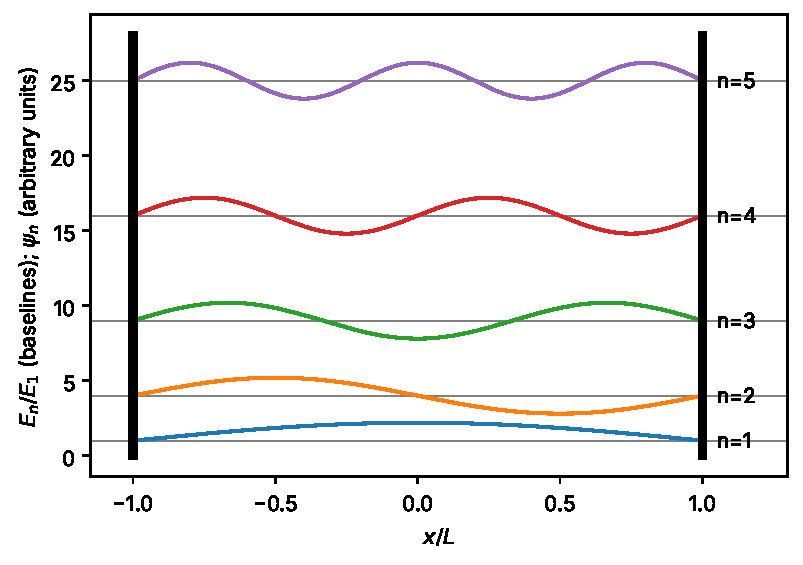
\includegraphics[width=0.85\linewidth]{figs/bound-states_box.pdf}
\caption{The first five states of the infinite square well on $[-L,L]$. Each wavefunction is drawn on a baseline at its energy $E_n/E_1=n^2$ (gray lines), with $E_1=(\pi/2L)^2$. The $n$-th state holds $n$ half-wavelengths and has $n-1$ nodes; odd $n$ gives an even function, even $n$ an odd one. Thick lines: the Dirichlet walls.}
\label{fig:bound-states-box}
\end{figure}

\Cref{fig:bound-states-box} shows the first five states. Three patterns are visible, and the next section proves that they hold for every one-dimensional well: the energies are all different; the states are alternately even and odd; and the $n$-th state crosses zero $n-1$ times inside the box.

\subsection{Spacing}

From \cref{eq:bound-states-boxE},
\begin{equation}
E_{n+1}-E_n=\frac{\pi^2}{4L^2}\bigl[(n+1)^2-n^2\bigr]=\frac{(2n+1)\pi^2}{4L^2}=(2n+1)E_1 .
\label{eq:bound-states-boxgap}
\end{equation}
The spacing grows linearly with $n$: in a box, levels \emph{spread out} as you go up. Keep this in mind; the Riemann zeros do the opposite.

\begin{sample}{The empty box of the paper (RE3)}
The paper's scale-1 box has half-width $L=44.883$ (Sec.~II~B of \cite{soniR1}). With no potential inside (running example RE3), find (a) $E_1$, (b) $E_{500}$, (c) how many levels lie at or below $E=1000$, (d) $E_{501}-E_{500}$.

\textbf{Step 1:} $E_1=\pi^2/(4L^2)$. Here $L^2=44.883^2=2014.48$ and $4L^2=8057.94$, so $E_1=9.8696/8057.94=1.2248\times10^{-3}$.

\textbf{Step 2:} $E_{500}=500^2E_1=250000\times1.2248\times10^{-3}=306.2$.

\textbf{Step 3:} $E_n\le1000$ means $n\pi/(2L)\le\sqrt{1000}$, that is $n\le 2L\sqrt{1000}/\pi=89.766\times31.623/3.1416=903.6$. The largest integer is 903.

\textbf{Step 4:} By \cref{eq:bound-states-boxgap}, $E_{501}-E_{500}=1001\,E_1=1.226$.

\[
\boxed{E_1=1.2248\times10^{-3},\quad E_{500}=306.2,\quad 903 \text{ levels } \le 1000,\quad E_{501}-E_{500}=1.226}
\]
In the paper, the Wu--Sprung potential fills this box. We will see in \cref{sec:bound-states-paper} that the filled box holds far fewer levels below 1000.
\end{sample}

\begin{sample}{Where is the particle?}
In the ground state of the box, what is the probability of finding the particle in the middle half, $-L/2<x<L/2$?

\textbf{Step 1:} By the Born rule, $P=\int_{-L/2}^{L/2}\psi_1^2\,\dd x=\frac1L\int_{-L/2}^{L/2}\cos^2\frac{\pi x}{2L}\,\dd x$.

\textbf{Step 2:} Use $\cos^2\theta=\tfrac12(1+\cos2\theta)$: $P=\frac{1}{2L}\int_{-L/2}^{L/2}\bigl(1+\cos\frac{\pi x}{L}\bigr)\dd x$.

\textbf{Step 3:} The first term gives $\frac{1}{2L}\cdot L=\frac12$.

\textbf{Step 4:} The second gives $\frac{1}{2L}\cdot\frac{L}{\pi}\bigl[\sin\frac{\pi x}{L}\bigr]_{-L/2}^{L/2}=\frac{1}{2\pi}\bigl(\sin\frac{\pi}{2}-\sin(-\frac{\pi}{2})\bigr)=\frac1\pi$.

\[
\boxed{P=\tfrac12+\tfrac1\pi\approx0.818}
\]
A classical particle bouncing at constant speed would spend exactly half its time in the middle half. The quantum ground state piles probability in the center. (Problem 31 shows that for high $n$ the answer returns to $\tfrac12$, as the correspondence principle requires.)
\end{sample}

\begin{checkpoint}
If you double the half-width $L$ of the box, what happens to $E_1$ and to every spacing $E_{n+1}-E_n$?
\end{checkpoint}
\checkanswer{Both scale as $1/L^2$ by \cref{eq:bound-states-boxE,eq:bound-states-boxgap}, so both drop to one quarter. A bigger box means longer wavelengths and lower energies.}

\begin{keyideas}
\item Box on $[-L,L]$ with Dirichlet walls: $E_n=(n\pi/2L)^2$, $\psi_n=L^{-1/2}\sin\bigl(n\pi(x+L)/2L\bigr)$, $n=1,2,\dots$
\item Odd $n$: even cosine states; even $n$: odd sine states. The states are orthonormal.
\item Box spacing $(2n+1)E_1$ grows with $n$: levels spread out.
\end{keyideas}

%==========================================================
\section{Uniqueness, parity and nodes}\label{sec:bound-states-parity}

\subsection{One-dimensional bound states are never degenerate}

Two different states with the same energy are called \emph{degenerate}. In three dimensions degeneracy is common (think of the hydrogen atom). In one dimension it never happens for bound states. The proof uses one fact about differential equations that we take on trust.

\begin{beyond}
\textbf{Taken on trust: uniqueness for the initial-value problem.} If $V$ is continuous on an interval and $x_0$ is a point in it, then for any numbers $a$, $b$ there is exactly one solution of $\psi''=(V-E)\psi$ on the interval with $\psi(x_0)=a$ and $\psi'(x_0)=b$. In particular, a solution with $\psi(x_0)=\psi'(x_0)=0$ is identically zero. This is the existence and uniqueness theorem for linear second-order equations; see \cite{rhb}. Physically: knowing the position and slope of the wavefunction at one point, the curvature rule \cref{eq:bound-states-curv} determines the rest, just as knowing a projectile's position and velocity determines its path.
\end{beyond}

\textbf{Theorem (proved, given the box above).} If $\psi_1$ and $\psi_2$ are bound states of the same potential with the same energy $E$, then $\psi_2=c\,\psi_1$ for a constant $c$.

\emph{Proof.} Define the \emph{Wronskian} $W(x)=\psi_1\psi_2'-\psi_2\psi_1'$.

\emph{Step 1: $W$ is constant.} By the product rule,
\[
W'=\psi_1'\psi_2'+\psi_1\psi_2''-\psi_2'\psi_1'-\psi_2\psi_1''=\psi_1\psi_2''-\psi_2\psi_1'' .
\]
Insert $\psi_i''=(V-E)\psi_i$ from \cref{eq:bound-states-curv}:
\[
W'=\psi_1(V-E)\psi_2-\psi_2(V-E)\psi_1=0 .
\]

\emph{Step 2: $W=0$.} At a Dirichlet wall $x=L$ both functions vanish, so $W(L)=0$. For a potential on the whole line, both $\psi_i$ and $\psi_i'$ tend to zero at infinity, so $W\to0$. Either way, the constant is zero.

\emph{Step 3: compare at one point.} Pick a point $x_0$ with $\psi_1(x_0)\ne0$ (one exists, since $\psi_1$ is not identically zero) and set $c=\psi_2(x_0)/\psi_1(x_0)$. Define $\phi=\psi_2-c\psi_1$, which solves the same equation (linearity). Then $\phi(x_0)=\psi_2(x_0)-c\psi_1(x_0)=0$.

\emph{Step 4: the slope also vanishes.} From $W(x_0)=0$: $\psi_1(x_0)\psi_2'(x_0)=\psi_2(x_0)\psi_1'(x_0)$. Divide by $\psi_1(x_0)$: $\psi_2'(x_0)=c\,\psi_1'(x_0)$. Hence $\phi'(x_0)=\psi_2'(x_0)-c\psi_1'(x_0)=0$.

\emph{Step 5.} By uniqueness, $\phi\equiv0$, so $\psi_2=c\psi_1$. $\square$

\subsection{Even potentials have even and odd states}

A potential is \emph{even} if $V(-x)=V(x)$: its graph is a mirror image about $x=0$. The box on $[-L,L]$, the oscillator $V=x^2$, and the paper's Wu--Sprung potential are all even.

\textbf{Theorem (proved).} If $V$ is even (and the region and boundary conditions are symmetric under $x\to-x$), every bound state is either even, $\psi(-x)=\psi(x)$, or odd, $\psi(-x)=-\psi(x)$.

\emph{Proof.}

\emph{Step 1: the mirror image is a solution.} Let $\psi$ solve \cref{eq:bound-states-tise} and define $\chi(x)=\psi(-x)$. By the chain rule, $\chi'(x)=-\psi'(-x)$ and $\chi''(x)=\psi''(-x)$ (two factors of $-1$ cancel). So
\[
-\chi''(x)+V(x)\chi(x)=-\psi''(-x)+V(-x)\psi(-x)=E\psi(-x)=E\chi(x),
\]
where the first equality used $V(x)=V(-x)$ and the second is \cref{eq:bound-states-tise} evaluated at the point $-x$. Also $\chi$ is normalizable and satisfies the mirrored boundary conditions, which are the same conditions. So $\chi$ is a bound state with energy $E$.

\emph{Step 2: nondegeneracy.} By the previous theorem, $\chi=c\psi$, that is $\psi(-x)=c\psi(x)$ for all $x$.

\emph{Step 3: $c=\pm1$.} Apply Step 2 twice: $\psi(x)=\psi(-(-x))=c\,\psi(-x)=c^2\psi(x)$. Since $\psi\ne0$ somewhere, $c^2=1$, so $c=1$ (even) or $c=-1$ (odd). $\square$

Two consequences are used again and again.
\begin{itemize}
\item An odd state has $\psi(0)=0$, because $\psi(0)=-\psi(0)$. An even state has $\psi'(0)=0$, because the derivative of an even function is odd.
\item For either parity, $\psi^2$ is even. So the probability density is symmetric, the particle is equally likely to be on either side, and $\langle x\rangle=\int x\psi^2\,\dd x=0$ (an odd integrand over a symmetric interval).
\end{itemize}

\subsection{Counting nodes}

A \emph{node} is a point strictly inside the region where $\psi$ crosses zero. In \cref{fig:bound-states-box} the $n$-th box state has $n-1$ nodes. This is a general law.

\begin{beyond}
\textbf{Taken on trust: the oscillation (node) theorem.} For a one-dimensional confining potential, the $n$-th bound state ($n=1$ the ground state) has exactly $n-1$ nodes. The proof uses Sturm's comparison method from the theory of Sturm--Liouville problems (see \cite{rhb} for that theory). Intuitively, raising $E$ makes $\psi''=(V-E)\psi$ curve more strongly, so the wavefunction turns over more often, and each additional allowed state squeezes in one more node.
\end{beyond}

Combine the node theorem with parity. In an even potential:
\begin{itemize}
\item An odd state has a node at $x=0$, and its other nodes come in pairs $\pm x_j$. So it has an \emph{odd} number of nodes.
\item An even state cannot have a node at $x=0$: it would have $\psi(0)=0$ and $\psi'(0)=0$, hence be identically zero by uniqueness. Its nodes come in pairs, so it has an \emph{even} number of nodes.
\end{itemize}
State $n$ has $n-1$ nodes. Therefore state $n$ is even when $n-1$ is even, that is when $n$ is odd, and odd when $n$ is even. The ground state of an even well is even (no nodes), and the parities then alternate: even, odd, even, odd, \dots. The box confirms this: odd $n$ gave cosines.

\begin{sample}{Parity and nodes of the third box state}
Find the parity and the nodes of $\psi_3$ in the box on $[-L,L]$, and check both general theorems.

\textbf{Step 1:} $n=3$ is odd, so by \cref{eq:bound-states-boxpsi} $\psi_3=L^{-1/2}\cos(3\pi x/2L)$, an even function.

\textbf{Step 2:} Nodes: $\cos(3\pi x/2L)=0$ when $3\pi x/2L=\pm\pi/2$ (the next zeros, $\pm3\pi/2$, give $x=\pm L$, the walls, which are not interior). So $x=\pm L/3$.

\textbf{Step 3:} Two nodes $=n-1$, as the node theorem demands; an even number, as an even state must have; none at $x=0$.

\[
\boxed{\psi_3 \text{ is even, with nodes at } x=\pm L/3}
\]
\end{sample}

\begin{checkpoint}
In an even potential, can the ground state be odd? How many nodes does the seventh state have, and what is its parity?
\end{checkpoint}
\checkanswer{No: an odd state has a node at $x=0$, but the ground state has none. The seventh state has $7-1=6$ nodes, an even number, so it is even.}

\begin{keyideas}
\item One-dimensional bound states are nondegenerate (Wronskian proof).
\item In an even potential each state is even or odd; odd states vanish at $x=0$, even states have zero slope there; $\psi^2$ is always even.
\item The $n$-th state has $n-1$ nodes (taken on trust); in an even well, odd $n$ means even state and even $n$ means odd state.
\end{keyideas}

%==========================================================
\section{The harmonic oscillator}\label{sec:bound-states-sho}

\subsection{The equation}

The harmonic oscillator is the quantum version of the mass on a spring. In ordinary units its potential is $\tfrac12m\omega^2x^2$. In our units $m=\tfrac12$, so the potential is $\tfrac14\omega^2x^2$. The simplest choice is $\omega=2$, which gives
\begin{equation}
-\psi''+x^2\psi=E\psi .
\label{eq:bound-states-sho}
\end{equation}
Any other strength reduces to this one by a change of scale (Sample Problem ``Stretching the oscillator'' below).

\subsection{Peeling off the Gaussian}

For large $|x|$ the term $x^2\psi$ dominates $E\psi$. Try $e^{-x^2/2}$: its derivative is $-xe^{-x^2/2}$ and its second derivative is $(x^2-1)e^{-x^2/2}$, so $-\psi''+x^2\psi=e^{-x^2/2}$, which is \cref{eq:bound-states-sho} with $E=1$. We have already found a bound state! To find the rest, write
\begin{equation}
\psi(x)=h(x)\,e^{-x^2/2}
\label{eq:bound-states-hsub}
\end{equation}
and find the equation for $h$. By the product rule,
\begin{align*}
\psi'&=\bigl(h'-xh\bigr)e^{-x^2/2},\\
\psi''&=\bigl(h''-h-xh'\bigr)e^{-x^2/2}-x\bigl(h'-xh\bigr)e^{-x^2/2}\\
&=\bigl(h''-2xh'-h+x^2h\bigr)e^{-x^2/2}.
\end{align*}
(In the second line the first bracket is the derivative of $h'-xh$; the second term is $h'-xh$ times the derivative $-x$ of the exponent.) So
\[
-\psi''+x^2\psi=\bigl(-h''+2xh'+h-x^2h+x^2h\bigr)e^{-x^2/2}=\bigl(-h''+2xh'+h\bigr)e^{-x^2/2}.
\]
Setting this equal to $Eh\,e^{-x^2/2}$ and dividing by $-e^{-x^2/2}$ gives \emph{Hermite's equation}
\begin{equation}
h''-2xh'+(E-1)h=0 .
\label{eq:bound-states-hermite}
\end{equation}

\subsection{Power series and the recursion}

Look for $h$ as a power series $h(x)=\sum_{j=0}^{\infty}a_jx^j$. Term by term,
\[
h'=\sum_{j}ja_jx^{j-1},\qquad h''=\sum_{j}j(j-1)a_jx^{j-2}.
\]
In $h''$ rename the index $j\to j+2$, so that every sum runs over powers $x^j$:
\[
h''=\sum_{j=0}^{\infty}(j+2)(j+1)a_{j+2}x^{j},\qquad -2xh'=\sum_{j=0}^{\infty}(-2j)a_jx^j .
\]
Insert into \cref{eq:bound-states-hermite}:
\[
\sum_{j=0}^{\infty}\Bigl[(j+2)(j+1)a_{j+2}-2ja_j+(E-1)a_j\Bigr]x^j=0 .
\]
A power series that vanishes for all $x$ has every coefficient zero, so
\begin{equation}
a_{j+2}=\frac{2j+1-E}{(j+2)(j+1)}\,a_j .
\label{eq:bound-states-recur}
\end{equation}
Choosing $a_0$ starts a chain of even powers; choosing $a_1$ starts a chain of odd powers. Even potential, even and odd solutions: exactly as the parity theorem promised.

\subsection{Quantization: the series must stop}

Suppose the chain never stops. For large $j$, \cref{eq:bound-states-recur} gives $a_{j+2}/a_j\approx 2j/j^2=2/j$. Compare $e^{x^2}=\sum_{k}x^{2k}/k!$: with $j=2k$, the ratio of successive coefficients is $\frac{1/(k+1)!}{1/k!}=\frac{1}{k+1}=\frac{2}{j+2}\approx\frac{2}{j}$. So a nonterminating $h$ grows at large $|x|$ like $e^{x^2}$, and then $\psi=he^{-x^2/2}$ grows like $e^{+x^2/2}$: not normalizable. This is the growing branch that wrecked the shooting curves in \cref{fig:bound-states-shooting}. (This standard comparison of tails is a heuristic as written; a careful version bounds the coefficients from below for all large $j$. See \cite{griffiths}.)

The only escape is for the chain to stop. The numerator of \cref{eq:bound-states-recur} vanishes at $j=J$ when $E=2J+1$; then $a_{J+2}=a_{J+4}=\cdots=0$ and $h$ is a polynomial of degree $J$. (The \emph{other} chain must be switched off by setting its starting coefficient to zero.) With our labeling $n=J+1$ starting from the ground state $n=1$:
\begin{equation}
E_n=2n-1,\qquad n=1,2,3,\dots
\label{eq:bound-states-shoE}
\end{equation}
The levels $1,3,5,7,\dots$ are \emph{equally spaced}, with spacing 2. The polynomial $h$ for level $n$ is, up to a constant, the Hermite polynomial $H_{n-1}$:
\[
H_0=1,\quad H_1=2x,\quad H_2=4x^2-2,\quad H_3=8x^3-12x .
\]
For example, $E=5$ ($J=2$): with $a_1=0$, \cref{eq:bound-states-recur} gives $a_2=\frac{1-5}{2}a_0=-2a_0$ and $a_4=0$, so $h=a_0(1-2x^2)$, proportional to $H_2$.

\begin{pitfall}
Most quantum texts label oscillator levels from zero, $E_\nu=\hbar\omega(\nu+\tfrac12)$, $\nu=0,1,2,\dots$ In this book, as in the paper, level indices start at $n=1$, so the ground state is $n=1$ and $E_n=2n-1$ in our units. With $\hbar=1$ and $\omega=2$, $\hbar\omega(\nu+\tfrac12)=2\nu+1=2n-1$ for $\nu=n-1$: the same numbers, a different label.
\end{pitfall}

\subsection{Normalizing: the Gaussian integral}

\begin{beyond}
\textbf{Taken on trust: the Gaussian integral.} $\displaystyle\int_{-\infty}^{\infty}e^{-x^2}\,\dd x=\sqrt\pi$. A short proof squares the integral, writes it as a double integral over the plane, and switches to polar coordinates; it needs double integrals, which this book does not assume. You can confirm it numerically: \texttt{scipy.integrate.quad(lambda x: np.exp(-x**2), -np.inf, np.inf)} returns $1.7724539\ldots=\sqrt\pi$.
\end{beyond}

From it, integration by parts gives the moments we need. With $u=x$ and $\dd v=xe^{-x^2}\dd x$ (so $v=-\tfrac12e^{-x^2}$):
\begin{equation}
\int_{-\infty}^{\infty}x^2e^{-x^2}\dd x=\Bigl[-\tfrac12xe^{-x^2}\Bigr]_{-\infty}^{\infty}+\tfrac12\int_{-\infty}^{\infty}e^{-x^2}\dd x=\frac{\sqrt\pi}{2},
\label{eq:bound-states-m2}
\end{equation}
since $xe^{-x^2}\to0$ at both ends. With $u=x^3$ and the same $\dd v$:
\begin{equation}
\int_{-\infty}^{\infty}x^4e^{-x^2}\dd x=\tfrac32\int_{-\infty}^{\infty}x^2e^{-x^2}\dd x=\frac{3\sqrt\pi}{4}.
\label{eq:bound-states-m4}
\end{equation}
So the ground state is $\psi_1=\pi^{-1/4}e^{-x^2/2}$, since $\int\psi_1^2\dd x=\pi^{-1/2}\int e^{-x^2}\dd x=1$.

\begin{sample}{Checking an oscillator state}
Show that $\psi(x)=(2x^2-1)e^{-x^2/2}$ solves \cref{eq:bound-states-sho}, find its energy and level index, normalize it, and locate its nodes and classical turning points.

\textbf{Step 1:} Here $h=2x^2-1$, $h'=4x$, $h''=4$. Insert into \cref{eq:bound-states-hermite}: $4-2x(4x)+(E-1)(2x^2-1)=\bigl[2(E-1)-8\bigr]x^2+\bigl[4-(E-1)\bigr]$.

\textbf{Step 2:} Both brackets vanish if and only if $E=5$. So $\psi$ is a solution with $E=5$, which is $2n-1$ with $n=3$: the third level.

\textbf{Step 3:} $\int(2x^2-1)^2e^{-x^2}\dd x=\int(4x^4-4x^2+1)e^{-x^2}\dd x=4\cdot\frac{3\sqrt\pi}{4}-4\cdot\frac{\sqrt\pi}{2}+\sqrt\pi=2\sqrt\pi$, using \cref{eq:bound-states-m2,eq:bound-states-m4}. So $\psi_3=(2\sqrt\pi)^{-1/2}(2x^2-1)e^{-x^2/2}$.

\textbf{Step 4:} Nodes where $2x^2-1=0$: $x=\pm1/\sqrt2=\pm0.7071$. Two nodes, $n-1=2$. Even function, as $n=3$ odd requires.

\textbf{Step 5:} Turning points where $x^2=E=5$: $x=\pm\sqrt5=\pm2.2361$.

\[
\boxed{E_3=5,\quad \psi_3=\frac{(2x^2-1)e^{-x^2/2}}{(2\sqrt\pi)^{1/2}},\quad \text{nodes } \pm0.7071,\quad \text{turning points } \pm2.2361}
\]
\end{sample}

\begin{figure}[htbp]\centering
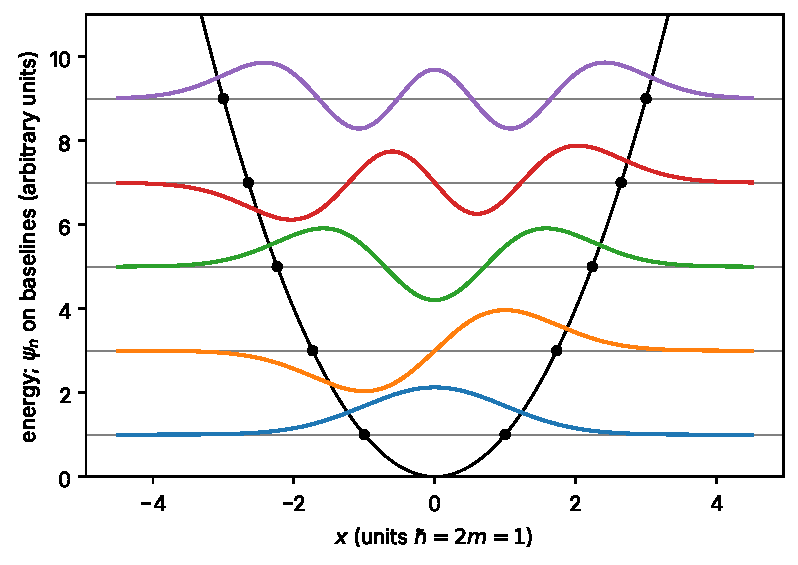
\includegraphics[width=0.85\linewidth]{figs/bound-states_oscillator.pdf}
\caption{The harmonic oscillator $V=x^2$ (units $\hbar=2m=1$). The first five normalized states are drawn on baselines at their energies $E_n=2n-1$. Dots mark the classical turning points $x=\pm\sqrt{E_n}$. Each state leaks a little past its turning points into the forbidden region, and the levels are equally spaced.}
\label{fig:bound-states-oscillator}
\end{figure}

\begin{sample}{Stretching the oscillator}
Find the levels of $-\psi''+ax^2\psi=E\psi$ for any $a>0$, and evaluate them for $a=\tfrac14$.

\textbf{Step 1:} Change variable $x=\beta y$ with $\beta>0$ to be chosen. By the chain rule $d/dx=(1/\beta)\,d/dy$, so $d^2\psi/dx^2=(1/\beta^2)\,d^2\psi/dy^2$. The equation becomes
\[
-\frac{1}{\beta^2}\frac{d^2\psi}{dy^2}+a\beta^2y^2\psi=E\psi .
\]

\textbf{Step 2:} Choose $\beta$ so that the two coefficients are equal: $a\beta^2=1/\beta^2$, that is $\beta^4=1/a$. Then
\[
\frac{1}{\beta^2}\Bigl(-\frac{d^2\psi}{dy^2}+y^2\psi\Bigr)=E\psi,\qquad\text{so}\qquad -\frac{d^2\psi}{dy^2}+y^2\psi=\beta^2E\,\psi .
\]

\textbf{Step 3:} This is \cref{eq:bound-states-sho} in the variable $y$, so $\beta^2E=2n-1$, and $1/\beta^2=\sqrt a$:
\[
E_n=\sqrt a\,(2n-1).
\]

\textbf{Step 4:} For $a=\tfrac14$: $E_n=\tfrac12(2n-1)=0.5,\,1.5,\,2.5,\dots$ This is $\tfrac14\omega^2x^2$ with $\omega=1$, and the result is $\omega(n-\tfrac12)$, the familiar $\hbar\omega(\nu+\tfrac12)$.

\[
\boxed{E_n=\sqrt a\,(2n-1);\quad a=\tfrac14:\ E_n=0.5,\ 1.5,\ 2.5,\dots}
\]
\end{sample}

You can confirm \cref{eq:bound-states-shoE} on a computer with the tridiagonal matrix of Chapter~\ref{ch:eigen}. Chapter~\ref{ch:finite-differences} analyzes this method in depth; here we use it as a black box.

\begin{pycode}
import numpy as np
from scipy.linalg import eigh_tridiagonal

L, N = 8.0, 2000                # box half-width, number of interior points
h = 2*L/(N + 1)                 # grid spacing
x = -L + h*np.arange(1, N + 1)  # interior grid points
V = x**2                        # oscillator potential, units hbar = 2m = 1
diag = 2/h**2 + V               # diagonal: second difference plus V
off = -np.ones(N - 1)/h**2      # off-diagonal of the second difference
E = eigh_tridiagonal(diag, off, eigvals_only=True,
                     select='i', select_range=(0, 9))
exact = 2*np.arange(1, 11) - 1  # 1, 3, 5, ..., 19
print(E)
print(E - exact)                # small, and growing with n
\end{pycode}

The walls at $x=\pm8$ lie far beyond the turning points of the first ten levels (the tenth has $E=19$ and turns at $\sqrt{19}\approx4.4$), so the box barely matters. The small differences that you see, below $0.01$ for all ten levels and growing with $n$, come from the grid, not the walls; Chapter~\ref{ch:finite-differences} explains them.

\begin{checkpoint}
If the oscillator potential $x^2$ is replaced by $4x^2$, what happens to the level spacing?
\end{checkpoint}
\checkanswer{With $a=4$, $E_n=2(2n-1)$, so the spacing becomes 4: it doubles. A stiffer spring vibrates at twice the angular frequency, and the spacing is $\hbar\omega$.}

\begin{keyideas}
\item $-\psi''+x^2\psi=E\psi$ has $E_n=2n-1$ and $\psi_n\propto H_{n-1}(x)e^{-x^2/2}$; the levels are equally spaced.
\item Quantization comes from requiring the power series to terminate; otherwise $\psi$ grows like $e^{x^2/2}$.
\item Scaling: $V=ax^2$ gives $E_n=\sqrt a(2n-1)$.
\end{keyideas}

%==========================================================
\section{The shape of a state in a general well}\label{sec:bound-states-shape}

Most wells, including the paper's, cannot be solved in closed form. The curvature rule still tells us what the states look like, and it tells us when a distant wall can be ignored.

\subsection{Reading a wavefunction}

Pick a level $E$ in a smooth, even, confining well. The turning points are $\pm x_E$, where $V(x_E)=E$.

\emph{Between the turning points} $\psi$ oscillates. Where $E-V$ is large (near the bottom of the well) the curvature is strong and the wiggles are short; near the turning points $E-V$ is small and the wiggles stretch out. The de Broglie relation (Chapter~\ref{ch:schrodinger}) makes this quantitative. Classically, in our units the kinetic energy is $p^2/2m=p^2$ (since $2m=1$), so $p(x)=\sqrt{E-V(x)}$ and the local wavelength is
\begin{equation}
\lambda(x)=\frac{2\pi\hbar}{p(x)}=\frac{2\pi}{\sqrt{E-V(x)}} .
\label{eq:bound-states-lambda}
\end{equation}
The amplitude also varies: it is larger where the particle is slow. A classical particle spends time $\dd t=\dd x/v$ in each slice $\dd x$, so its classical probability density is proportional to $1/v$; the quantum density, averaged over the wiggles, follows this trend for high levels. In \cref{fig:bound-states-oscillator} the high states are largest near their turning points, where a classical oscillator is slowest.

\emph{Beyond the turning points} $\psi$ decays. The local decay rate is $\kappa(x)=\sqrt{V(x)-E}$; the farther above $E$ the potential rises, the faster the decay. The wavefunction does \emph{not} vanish at the turning point; it leaks into the forbidden region (look at \cref{fig:bound-states-oscillator}).

\begin{pitfall}
The classical turning point is not a node. The wavefunction is continuous and smooth there; it merely changes from curving toward the axis to curving away. A quantum particle has a nonzero probability of being found in the classically forbidden region (Problem 13 computes it for the oscillator ground state).
\end{pitfall}

\subsection{How much does a distant wall matter?}

The paper puts its Wu--Sprung potential in a box. A wall placed far into the forbidden region should change the levels very little, since $\psi$ is already tiny there. Let us estimate how little, using the oscillator, where everything is known.

\begin{sample}{How much does a distant wall matter?}
Put the oscillator \cref{eq:bound-states-sho} inside Dirichlet walls at $\pm L$, with $L$ larger than the turning point $x=1$ of the ground state. Estimate the rise of the ground-state energy above 1.

\textbf{Step 1 (two equations):} Let $\psi=\pi^{-1/4}e^{-x^2/2}$ be the ground state without walls, energy 1, and $\phi$ the ground state with walls, energy $E_b$, $\phi(\pm L)=0$. Then
\[
-\psi''+x^2\psi=\psi,\qquad -\phi''+x^2\phi=E_b\phi .
\]

\textbf{Step 2 (combine):} Multiply the second by $\psi$, the first by $\phi$, and subtract; the $x^2$ terms cancel:
\[
\psi''\phi-\phi''\psi=(E_b-1)\phi\psi .
\]

\textbf{Step 3 (total derivative):} By the product rule, $\frac{d}{dx}(\psi'\phi-\phi'\psi)=\psi''\phi+\psi'\phi'-\phi''\psi-\phi'\psi'=\psi''\phi-\phi''\psi$.

\textbf{Step 4 (integrate from $-L$ to $L$):} $\bigl[\psi'\phi-\phi'\psi\bigr]_{-L}^{L}=(E_b-1)\int_{-L}^{L}\phi\psi\,\dd x$. Since $\phi(\pm L)=0$ the left side is $-\phi'(L)\psi(L)+\phi'(-L)\psi(-L)$. Both states are even, so $\psi(-L)=\psi(L)$ and $\phi'(-L)=-\phi'(L)$, and the left side is $-2\phi'(L)\psi(L)$. This step is exact:
\begin{equation}
E_b-1=\frac{-2\phi'(L)\psi(L)}{\int_{-L}^{L}\phi\psi\,\dd x}.
\label{eq:bound-states-green}
\end{equation}

\textbf{Step 5 (approximate, heuristic):} The two states differ only near the walls, where both are tiny, so $\int\phi\psi\,\dd x\approx1$. Near $x=L$, $\phi$ is $\psi$ minus just enough of the growing solution to make it vanish at the wall. In the forbidden region, the decaying solution has $\psi'/\psi=-x$ exactly, and the growing one behaves like $e^{+x^2/2}$, with logarithmic slope close to $+x$. So $\phi'(L)\approx\psi'(L)-L\psi(L)=-L\psi(L)-L\psi(L)=-2L\psi(L)$. This approximation requires $L^2\gg E$, so that the potential dominates near the wall.

\textbf{Step 6 (result):} $E_b-1\approx4L\psi(L)^2=\dfrac{4L}{\sqrt\pi}e^{-L^2}$.

\textbf{Step 7 (numbers):} For $L=2$: $\frac{8}{\sqrt\pi}e^{-4}=0.083$. A numerical solution (the tridiagonal method above) gives $E_b\approx1.075$, so the estimate is about 10\% high, reasonable since $L^2=4$ is only four times $E$. For $L=4$: $\frac{16}{\sqrt\pi}e^{-16}\approx1.0\times10^{-6}$, and numerically the shift is below $10^{-5}$.

\[
\boxed{E_b-1\approx\frac{4L}{\sqrt\pi}e^{-L^2}:\ \ L=2\to0.083\ (\text{numerics }0.075),\ \ L=4\to\sim10^{-6}}
\]
\end{sample}

The lesson is general: the effect of a wall placed beyond a turning point falls off exponentially with the amount of forbidden region in between, roughly like $\psi(L)^2$. \Cref{fig:bound-states-wall} compares the estimate with numerics.

\begin{figure}[htbp]\centering
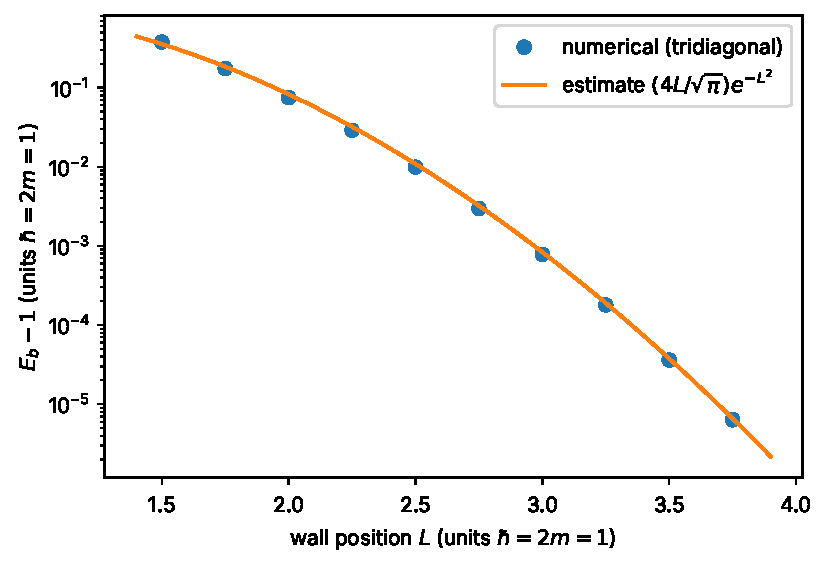
\includegraphics[width=0.85\linewidth]{figs/bound-states_wall.pdf}
\caption{Rise of the oscillator ground-state energy, $E_b-1$, when Dirichlet walls are placed at $\pm L$ (units $\hbar=2m=1$; logarithmic vertical axis). Dots: numerical eigenvalues of the tridiagonal matrix. Line: the estimate $(4L/\sqrt\pi)e^{-L^2}$ of \cref{eq:bound-states-green} and Step 6. The effect of the wall dies off like $e^{-L^2}$, the square of the wavefunction at the wall.}
\label{fig:bound-states-wall}
\end{figure}

\begin{keyideas}
\item Inside the allowed region the local wavelength is $2\pi/\sqrt{E-V}$; outside, the decay rate is $\sqrt{V-E}$.
\item Wavefunctions leak past turning points; turning points are not nodes.
\item A Dirichlet wall deep in the forbidden region shifts a level by an amount that is exponentially small (for the oscillator ground state, about $(4L/\sqrt\pi)e^{-L^2}$).
\end{keyideas}

%==========================================================
\section{How the spacing depends on the shape of the well}\label{sec:bound-states-spacing}

The box has spacings that grow, $(2n+1)E_1$; the oscillator has constant spacing 2. What decides? We now build a simple counting rule that answers this for any well. It is a \emph{heuristic} here; Chapter~\ref{ch:wkb} derives it properly as the Bohr--Sommerfeld rule.

\subsection{Counting half-wavelengths}

In the box, the $n$-th state holds exactly $n$ half-wavelengths. In a general well the wavelength \cref{eq:bound-states-lambda} varies with position, so count half-wavelengths piece by piece: a slice of width $\dd x$ contains $\dd x/(\lambda/2)=\sqrt{E-V}\,\dd x/\pi$ of them. Adding up the slices between the turning points $x_1$ and $x_2$:
\begin{equation}
\frac1\pi\int_{x_1}^{x_2}\sqrt{E_n-V(x)}\,\dd x\;\approx\;n-\gamma .
\label{eq:bound-states-count}
\end{equation}
The constant $\gamma$ accounts for how the wavefunction meets the boundary. At a hard wall it is pinned to zero; at a soft turning point it leaks into the forbidden region, so the oscillation inside is a little short of a full extra half-wavelength. The precise result (Chapter~\ref{ch:wkb}) is $\gamma=0$ for two hard walls and $\gamma=\tfrac12$ for two soft turning points. Here we test the rule on wells we already know.

\emph{Box} (hard walls, $\gamma=0$): $V=0$ on $[-L,L]$, so $\frac1\pi\cdot2L\sqrt{E_n}=n$, which gives $E_n=(n\pi/2L)^2$. Exactly \cref{eq:bound-states-boxE}.

\emph{Oscillator} (soft turning points at $\pm\sqrt E$, $\gamma=\tfrac12$): substitute $x=\sqrt E\sin\theta$, $\dd x=\sqrt E\cos\theta\,\dd\theta$, with $\theta$ from $-\pi/2$ to $\pi/2$:
\[
\int_{-\sqrt E}^{\sqrt E}\sqrt{E-x^2}\,\dd x=E\int_{-\pi/2}^{\pi/2}\cos^2\theta\,\dd\theta=E\cdot\frac\pi2 .
\]
So \cref{eq:bound-states-count} reads $E_n/2=n-\tfrac12$, that is $E_n=2n-1$. Exactly \cref{eq:bound-states-shoE}. (For the oscillator this is a lucky exactness; for most wells the rule is only approximate.)

\subsection{Power-law wells}

Now take $V=|x|^\alpha$ with $\alpha>0$. The turning points are $\pm a$ with $a=E^{1/\alpha}$. Substitute $x=au$:
\[
\int_{-a}^{a}\sqrt{E-|x|^\alpha}\,\dd x=2a\int_0^1\sqrt{E-a^\alpha u^\alpha}\,\dd u=2a\sqrt E\int_0^1\sqrt{1-u^\alpha}\,\dd u=2E^{\frac1\alpha+\frac12}I_\alpha ,
\]
where $I_\alpha=\int_0^1\sqrt{1-u^\alpha}\,\dd u$ is a pure number and we used $a^\alpha=E$ and $a=E^{1/\alpha}$. The counting rule becomes
\begin{equation}
\frac{2I_\alpha}{\pi}E_n^{\frac12+\frac1\alpha}\approx n-\tfrac12,
\qquad\text{so}\qquad
E_n\propto\bigl(n-\tfrac12\bigr)^{\frac{2\alpha}{\alpha+2}}.
\label{eq:bound-states-powerlaw}
\end{equation}
Checks: $\alpha=2$ gives $I_2=\pi/4$ (a quarter of the unit disk) and $E_n\propto n$; as $\alpha\to\infty$ the well becomes a box of half-width 1, $I_\alpha\to1$, and $E_n\propto n^2$. In general the spacing behaves as
\[
E_{n+1}-E_n\approx\frac{dE_n}{dn}\propto n^{\frac{2\alpha}{\alpha+2}-1}=n^{\frac{\alpha-2}{\alpha+2}}:
\]
\begin{itemize}
\item $\alpha>2$ (walls steeper than a parabola): spacing \emph{grows} with $n$; the box is the extreme case.
\item $\alpha=2$: constant spacing.
\item $\alpha<2$ (walls gentler than a parabola): spacing \emph{shrinks}; the levels crowd together as you climb.
\end{itemize}

\subsection{The V-shaped well}

The linear well $V=|x|$ ($\alpha=1$) is exactly solvable with a special function.

\begin{beyond}
\textbf{Taken on trust: Airy functions.} For $x>0$, $-\psi''+x\psi=E\psi$ becomes $\psi''=y\psi$ with $y=x-E$. This is Airy's equation. Its solution that decays as $y\to+\infty$ is a named special function, $\mathrm{Ai}(y)$, which oscillates for $y<0$ and has zeros at $y=a_1>a_2>\cdots$ (all negative), while its derivative $\mathrm{Ai}'$ has zeros at $a'_1>a'_2>\cdots$. These are tabulated and available as \texttt{scipy.special.ai\_zeros}. Taking $\psi=\mathrm{Ai}(x-E)$ for $x>0$ and extending by parity: odd states need $\psi(0)=0$, so $E=-a_k$; even states need $\psi'(0)=0$, so $E=-a'_k$. The construction is complete except for the properties of $\mathrm{Ai}$, which we take from the tables.
\end{beyond}

\begin{table}[htbp]\centering
\caption{The first six levels of three even wells (units $\hbar=2m=1$). Box: half-width $L=\pi/2$, so $E_n=n^2$. Oscillator: $V=x^2$. V-shaped: $V=|x|$, levels from Airy zeros. The parity column holds for all three wells.}
\label{tab:bound-states-ladder}
\begin{tabular}{cccccc}
\toprule
$n$ & parity & nodes & box $L=\pi/2$ & $V=x^2$ & $V=|x|$\\
\midrule
1 & even & 0 & 1 & 1 & 1.0188\\
2 & odd  & 1 & 4 & 3 & 2.3381\\
3 & even & 2 & 9 & 5 & 3.2482\\
4 & odd  & 3 & 16 & 7 & 4.0879\\
5 & even & 4 & 25 & 9 & 4.8201\\
6 & odd  & 5 & 36 & 11 & 5.5206\\
\bottomrule
\end{tabular}
\end{table}

\begin{sample}{Counting half-wavelengths in a V-shaped well}
Use \cref{eq:bound-states-count} with $\gamma=\tfrac12$ to estimate $E_1$, $E_2$, $E_9$, $E_{10}$ of $V=|x|$, and compare with the Airy values.

\textbf{Step 1:} Here $\alpha=1$, $I_1=\int_0^1\sqrt{1-u}\,\dd u=\bigl[-\tfrac23(1-u)^{3/2}\bigr]_0^1=\tfrac23$. So \cref{eq:bound-states-powerlaw} gives $\frac{4}{3\pi}E_n^{3/2}=n-\tfrac12$, that is
\[
E_n\approx\Bigl[\tfrac{3\pi}{4}\bigl(n-\tfrac12\bigr)\Bigr]^{2/3}.
\]

\textbf{Step 2:} $n=1$: $(3\pi/8)^{2/3}=1.1781^{2/3}=1.115$. $n=2$: $3.5343^{2/3}=2.320$. $n=9$: $20.028^{2/3}=7.375$. $n=10$: $22.384^{2/3}=7.942$.

\textbf{Step 3:} Airy values: odd $n$ is even parity, so $E_n=-a'_{(n+1)/2}$; even $n$ is odd parity, $E_n=-a_{n/2}$. That gives $E_1=1.019$, $E_2=2.338$, $E_9=-a'_5=7.372$, $E_{10}=-a_5=7.944$.

\[
\boxed{\begin{array}{c|cccc} n&1&2&9&10\\\hline\text{counting}&1.115&2.320&7.375&7.942\\ \text{exact}&1.019&2.338&7.372&7.944\end{array}}
\]
The rule is off by about 10\% for the ground state and by less than $0.003$ at $n=9,10$. This is typical of semiclassical counting: weak for the lowest levels, excellent for high ones. The paper meets the same pattern: the Wu--Sprung construction is worst ``at low $n$, the known semiclassical weakness of the construction'' (Sec.~II~B of \cite{soniR1}).
\end{sample}

\begin{figure}[htbp]\centering
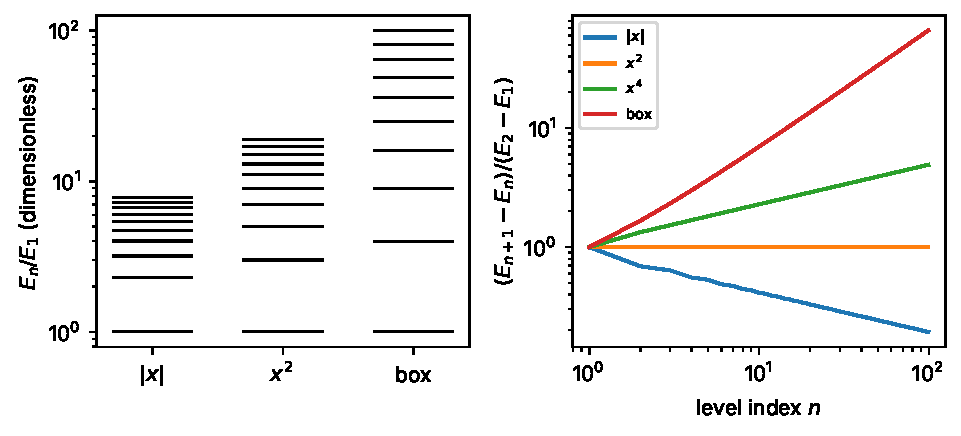
\includegraphics[width=0.95\linewidth]{figs/bound-states_ladders.pdf}
\caption{Left: the first ten levels of three even wells, scaled by their ground-state energy (logarithmic axis): $V=|x|$ (levels crowd), $V=x^2$ (equally spaced), and the box (levels spread). Right: spacing $E_{n+1}-E_n$, divided by the first spacing, versus $n$ on logarithmic axes, for $V=|x|$, $x^2$, $x^4$ and the box. The slopes approach $(\alpha-2)/(\alpha+2)$: $-1/3$, $0$, $1/3$ and $1$. Energies in units $\hbar=2m=1$; the scaled quantities are dimensionless.}
\label{fig:bound-states-ladders}
\end{figure}

\begin{checkpoint}
For $V=|x|^3$, do the levels crowd or spread as $n$ grows?
\end{checkpoint}
\checkanswer{They spread, slowly: $\alpha=3>2$, so $E_n\propto n^{6/5}$ and the spacing grows like $n^{1/5}$.}

\begin{keyideas}
\item Heuristic counting rule: $\frac1\pi\int\sqrt{E_n-V}\,\dd x\approx n-\gamma$ ($\gamma=0$ hard walls, $\tfrac12$ soft turning points); exact for the box and oscillator, accurate at high $n$ in general, weakest at low $n$.
\item For $V=|x|^\alpha$: $E_n\propto n^{2\alpha/(\alpha+2)}$. Steeper than a parabola: spacing grows. Gentler: spacing shrinks.
\end{keyideas}

%==========================================================
\section{Level density, and why slow growth means crowding}\label{sec:bound-states-density}

\subsection{Counting function and density}

When levels are numerous, it is convenient to describe them collectively. The \emph{counting function} $N(E)$ is the number of levels with $E_n\le E$. It is a staircase that jumps by 1 at each level. Its smooth trend $\bar N(E)$ is what the counting rule \cref{eq:bound-states-count} supplies:
\[
\bar N(E)=\frac1\pi\int_{x_1(E)}^{x_2(E)}\sqrt{E-V(x)}\,\dd x+\gamma ,
\]
with $\bar N(E_n)\approx n$ (the $\gamma$ is the same constant as before). The \emph{level density} is the derivative
\begin{equation}
\rho(E)=\frac{d\bar N}{dE},
\label{eq:bound-states-rho}
\end{equation}
the number of levels per unit energy near $E$. Its inverse $1/\rho$ is the \emph{mean spacing} near $E$.

\begin{pitfall}
The level density $\rho(E)$ counts levels per unit \emph{energy}; the probability density $|\psi(x)|^2$ is probability per unit \emph{length} for one state. They are unrelated quantities that share a name.
\end{pitfall}

\subsection{Density equals classical period over $2\pi$}

Differentiate $\bar N$. The limits $x_{1,2}(E)$ depend on $E$, so we need Leibniz's rule for differentiating an integral with variable limits: the derivative is the integral of the derivative of the integrand, plus the integrand at each limit times the rate at which that limit moves (with a minus sign at the lower limit) \cite{rhb}. At a turning point the integrand $\sqrt{E-V}$ is zero, so the limit terms vanish, and
\begin{equation}
\rho(E)=\frac1\pi\int_{x_1}^{x_2}\frac{\dd x}{2\sqrt{E-V(x)}}=\frac{1}{2\pi}\int_{x_1}^{x_2}\frac{\dd x}{\sqrt{E-V(x)}} .
\label{eq:bound-states-rho-int}
\end{equation}
(The integrand blows up at the turning points, but like $1/\sqrt{\text{distance}}$, which integrates to a finite value.) Now the classical meaning. With $m=\tfrac12$, kinetic energy is $\tfrac12mv^2=v^2/4=E-V$, so the classical speed is $v=2\sqrt{E-V}$. The time to cross from $x_1$ to $x_2$ is $\int\dd x/v$, and a full round trip takes twice that:
\[
T_{\rm cl}(E)=2\int_{x_1}^{x_2}\frac{\dd x}{2\sqrt{E-V}}=\int_{x_1}^{x_2}\frac{\dd x}{\sqrt{E-V}} .
\]
Comparing with \cref{eq:bound-states-rho-int}:
\begin{equation}
\rho(E)=\frac{T_{\rm cl}(E)}{2\pi},\qquad\text{equivalently}\qquad\text{mean spacing}=\frac{2\pi}{T_{\rm cl}}=\omega_{\rm cl}.
\label{eq:bound-states-period}
\end{equation}
In ordinary units this is $\Delta E\approx\hbar\omega_{\rm cl}$: the level spacing is $\hbar$ times the classical angular frequency of the orbit at that energy. This is a heuristic (semiclassical) result, accurate for high levels.

Check it against first-year physics. Simple harmonic motion has a period that does \emph{not} depend on amplitude, so the oscillator's spacing should be constant: for $V=x^2$, $\omega_{\rm cl}=2$ (from $\tfrac14\omega^2=1$), and the spacing is indeed 2. In the box a particle of speed $v=2\sqrt E$ makes a round trip of length $4L$ in time $T_{\rm cl}=4L/(2\sqrt E)=2L/\sqrt E$, so $\rho=L/(\pi\sqrt E)$; differentiating $\bar N=2L\sqrt E/\pi$ gives the same. For power laws, $\rho\propto E^{\frac1\alpha-\frac12}$ (differentiate \cref{eq:bound-states-powerlaw}).

\subsection{Why a slowly growing potential crowds its levels}

\Cref{eq:bound-states-period} gives the physical answer to the question of this section. A potential that grows slowly lets a more energetic particle travel much farther before turning around. If the distance it gains grows faster than its speed, its round trip takes \emph{longer} at higher energy, $T_{\rm cl}$ grows, $\rho$ grows, and the levels crowd together. A parabola is the borderline: the extra distance and the extra speed exactly balance and the period is constant. Steeper walls (the box) shorten the period as $E$ grows and spread the levels.

\subsection{The density of the Riemann zeros}

The smooth counting function of the zeta zeros is the paper's Eq.~(1) (derived in Chapter~\ref{ch:counting-zeros}):
\[
\Nsm(t)=\frac{t}{2\pi}\log\frac{t}{2\pi}-\frac{t}{2\pi}+\frac78 .
\]
Differentiate, using the product rule on the first term:
\[
\frac{d\Nsm}{dt}=\frac{1}{2\pi}\log\frac{t}{2\pi}+\frac{t}{2\pi}\cdot\frac1t-\frac{1}{2\pi}=\frac{1}{2\pi}\log\frac{t}{2\pi}.
\]
So if the zeros are to be the levels of a well, that well must have
\begin{equation}
\rho(E)=\frac{1}{2\pi}\log\frac{E}{2\pi},
\label{eq:bound-states-rhozeta}
\end{equation}
a density that \emph{grows}, but only logarithmically: from $0.129$ per unit at $t_1=14.13$ to $0.863$ at $t_{1000}=1419.42$. The levels crowd, so the classical period must grow with energy, so the potential must grow more slowly than a parabola. But the growth is gentle, so the potential is only a little slower than a parabola. \Cref{fig:bound-states-density} compares the densities.

\begin{figure}[htbp]\centering
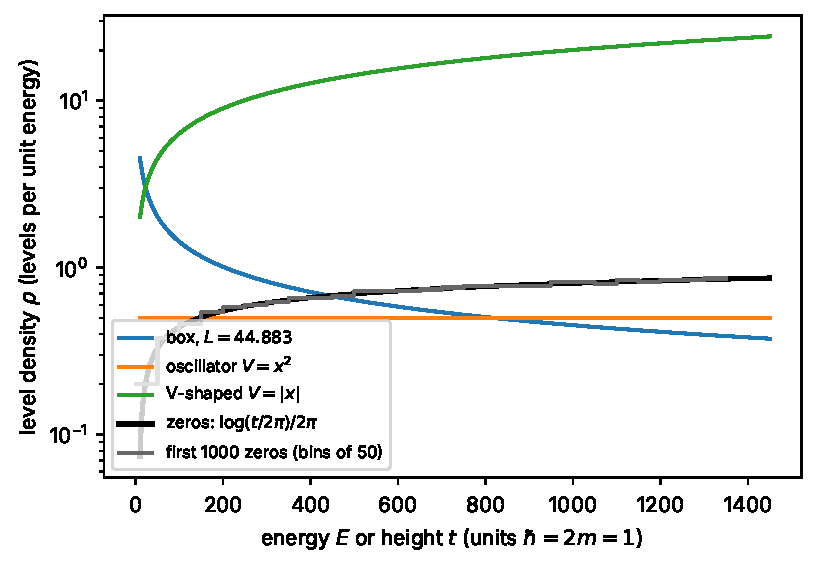
\includegraphics[width=0.85\linewidth]{figs/bound-states_density.pdf}
\caption{Level density $\rho(E)$ (levels per unit energy, logarithmic axis) versus energy (units $\hbar=2m=1$). Box with $L=44.883$: $L/(\pi\sqrt E)$, falling. Oscillator $V=x^2$: constant $\tfrac12$. V-shaped well $V=|x|$: $(2/\pi)\sqrt E$, rising fast. Riemann zeros: the smooth density $\frac{1}{2\pi}\log(t/2\pi)$ (line) and a histogram of the first 1000 zeros in bins of width 50 (steps). The zeros' density rises, but much more slowly than for the V-shaped well.}
\label{fig:bound-states-density}
\end{figure}

\begin{sample}{What shape of well do the zeros want?}
Treat the zeros' density as if it came locally from a power law $|x|^\alpha$, and find the effective exponent $\alpha$ near the 500th zero, $t_{500}=811.18$ (value from App.~A of \cite{soniR1}). Also find the mean spacing there and compare with the empty box of RE3.

\textbf{Step 1:} For a power law $\rho\propto E^{1/\alpha-1/2}$, so $\frac{d\log\rho}{d\log E}=\frac1\alpha-\frac12$.

\textbf{Step 2:} For \cref{eq:bound-states-rhozeta}, $\log\rho=\log\log\frac{t}{2\pi}-\log2\pi$. Since $\frac{d}{d\log t}=t\frac{d}{dt}$, the chain rule gives
\[
\frac{d\log\rho}{d\log t}=t\cdot\frac{1}{\log(t/2\pi)}\cdot\frac1t=\frac{1}{\log(t/2\pi)} .
\]

\textbf{Step 3:} At $t=811.18$: $t/2\pi=129.10$, $\log129.10=4.8606$, so $\frac{1}{\log(t/2\pi)}=0.2057$.

\textbf{Step 4:} $\frac1\alpha=\frac12+0.2057=0.7057$, so $\alpha=1.417$.

\textbf{Step 5:} Density $\rho=4.8606/(2\pi)=0.774$, mean spacing $1/\rho=1.293$. The empty box at the same energy has $\rho=L/(\pi\sqrt E)=44.883/(\pi\times28.481)=0.502$, spacing $1.99$.

\[
\boxed{\alpha_{\rm eff}\approx1.42 \text{ at } t\approx811;\quad \text{mean spacing } 1.293 \text{ (box: } 1.99)}
\]
The effective exponent lies between the V-shaped well ($\alpha=1$) and the parabola ($\alpha=2$), and since $1/\log(t/2\pi)\to0$ it creeps toward 2 as $t$ grows, but only logarithmically slowly. This is a heuristic local description, not an exact property of any potential.
\end{sample}

\begin{checkpoint}
The paper scores errors in units of the ``local mean spacing'' $\gap_n$ (Sec.~II~A of \cite{soniR1}). In the language of this section, what is $\gap_n$?
\end{checkpoint}
\checkanswer{It is $1/\rho$ evaluated at the $n$-th smooth zero, $2\pi/\log(s_n/2\pi)$: the average distance between neighboring levels at that height. Chapter~\ref{ch:counting-zeros} derives it.}

\begin{keyideas}
\item Counting function $N(E)$, smooth trend $\bar N(E)$, level density $\rho=d\bar N/dE$, mean spacing $1/\rho$.
\item Heuristic: $\rho=T_{\rm cl}/2\pi$; mean spacing $=\hbar\omega_{\rm cl}$.
\item Slowly growing potential $\Rightarrow$ longer classical period at higher energy $\Rightarrow$ crowding levels.
\item The zeros have $\rho=\frac1{2\pi}\log\frac{t}{2\pi}$: gently increasing, so their potential grows a little more slowly than a parabola (effective exponent about 1.4 near $t\approx800$).
\end{keyideas}

%==========================================================
\section{Paper connection}\label{sec:bound-states-paper}

\subsection{The box and its walls}

Section~II~B of \cite{soniR1} states the setting: ``In units $\hbar=2m=1$, $H=-d^2/dx^2+V(x)$ with $V$ even.'' The Wu--Sprung potential of Eq.~(2) is defined for $V\ge V_0=3.10073\pi\approx9.741$; it equals $V_0$ at $x=0$ (both terms of Eq.~(2) vanish when $V=V_0$, because $\sqrt{V-V_0}=0$ and the logarithm becomes $\log1$) and rises on both sides. The problem is posed on ``the domain $[-L,L]$ with $L=x(V{=}1000)=44.883$'' at scale 1 and $L=x(V{=}1500)=59.957$ at scale 2, with ``Dirichlet walls'' in the finite-difference solver. So the paper's operator is exactly the situation of this chapter: a smooth even well, closed off by the walls of \cref{sec:bound-states-box}. The empty box of RE3 (Sample Problem ``The empty box of the paper'') is what you get by deleting the potential.

Why are the walls harmless? The walls are placed where the potential has climbed to 1000 (scale 1). The scored levels are ``the first 500'' (Sec.~II~B), and the 500th zero is $t_{500}=811.1843588465$ (App.~A, key anchors). So every scored level lies well below the potential at the wall. By the reasoning of \cref{sec:bound-states-shape}, each scored state decays through a stretch of forbidden region before reaching the wall: for level 500 the turning point is at $x(811.18)\approx38.5$, about 6.4 units inside the wall at $44.883$, where $V-E$ climbs from 0 to about 190. The wall's influence on such a state is exponentially small, as \cref{fig:bound-states-wall} shows for the oscillator. Levels with energies close to 1000 would feel the wall strongly; the paper's solver computes more levels than it scores (App.~A step~4: eigenvalue range $[0,900]$ for the Hermitian work at scale 1).

\begin{figure}[htbp]\centering
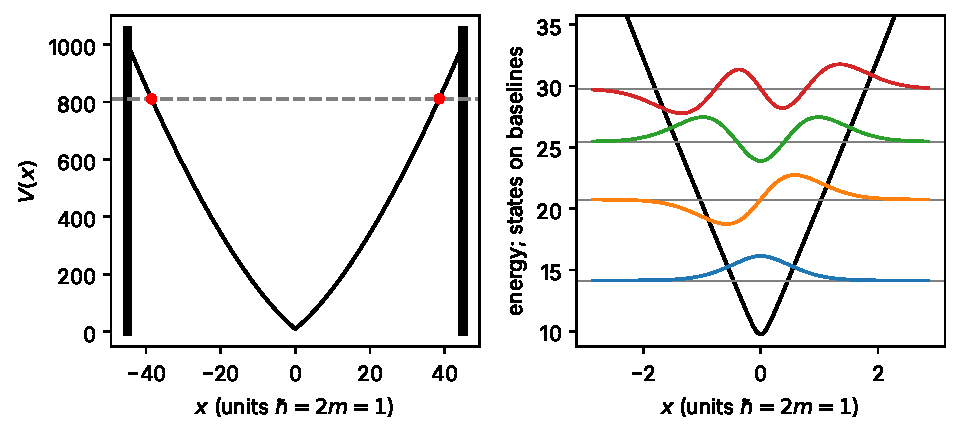
\includegraphics[width=0.95\linewidth]{figs/bound-states_wusprung.pdf}
\caption{The paper's scale-1 setting (units $\hbar=2m=1$). Left: the Wu--Sprung potential of Eq.~(2) of \cite{soniR1} on $[-L,L]$, $L=44.883$, with Dirichlet walls (thick lines) where $V=1000$. The dashed line is the energy $t_{500}=811.18$ of the last scored level; dots mark its turning points, about 6.4 units inside the walls. Right: close-up near the bottom of the well ($V_0\approx9.741$), with the first four eigenfunctions drawn on baselines at their computed energies; they alternate even, odd, even, odd and have $0,1,2,3$ nodes.}
\label{fig:bound-states-wusprung}
\end{figure}

\subsection{Counting levels in the filled box}

The empty box holds 903 levels at or below $E=1000$ (Sample Problem above). The paper reports 652 states with $E\le1000$ (Sec.~II~E and App.~A step~4: ``$[0,1000]$ (tensors; 652 states)''). The Wu--Sprung potential occupies the box and pushes the levels up, so far fewer fit below 1000. How many should fit? The potential was built so that its levels follow the smooth zeros, so the count should be close to $\Nsm(1000)+\tfrac12$, and $\Nsm(1000)=648.6$. The agreement is close but not exact; we do not analyze the small difference here (Problem 19 suggests one likely contributor).

\subsection{Level index and turning points}

The paper labels levels from $n=1$, as we do. Because the $n$-th state lives mostly between its turning points and is most sensitive to the potential there (Chapter~\ref{ch:perturbation} makes this precise), each level index corresponds to a position. Section~III (Interpolation split) uses exactly this: ``Position maps to level index through the classical turning point, and levels 201--300 turn at $x=22.5$--$28.5$.'' Figure~4 of the paper shades that band. Problem 22 asks you to reproduce these numbers.

\subsection{Why the potential is even, and what evenness buys}

The counting rule \cref{eq:bound-states-count} depends on the potential only through how much room the particle has at each energy, not on how that room is arranged. (The box on $[-L,L]$ and the box on $[0,2L]$ have identical levels; to leading semiclassical order, the same is true of any two wells whose allowed intervals have the same lengths at every energy.) So a list of levels cannot by itself fix the potential, and Wu and Sprung \cite{wusprung} fixed the ambiguity by choosing an even potential. Chapter~\ref{ch:wu-sprung} carries out the construction. Evenness has three consequences visible in the paper.
\begin{itemize}
\item \emph{Alternating parity.} By \cref{sec:bound-states-parity}, the states alternate even, odd, even, \dots, starting from an even ground state (\cref{fig:bound-states-wusprung}, right).
\item \emph{Even corrections.} The fitted correction $\delta V(x)=\sum_k c_k\cos(k\pi x/L)$ of Sec.~II~C uses even functions, and the alternative bases of Sec.~II~C, Chebyshev $T_k(2|x|/L-1)$ and hat functions of $|x|/L$, are even because they depend on $|x|$. So $V+\delta V$ stays even.
\item \emph{Odd perturbations have no diagonal elements.} Since $\psi_n^2$ is even, $\int\psi_n^2\,f\,\dd x=0$ for any odd $f$ (an odd integrand on a symmetric interval). The paper's PT-odd class uses $\phi_k=\sin((k+1)\pi x/L)$, which is odd, and Sec.~II~E notes ``$A_{nn}=0$'': this is exactly that parity fact (Problem 27). Conversely, for the Hermitian fit, the first-order sensitivity $A_{nk}=\int|\psi_n|^2\phi_k\,\dd x$ of Sec.~II~C would vanish for any odd basis function, so restricting $\delta V$ to even functions loses nothing at first order (Problem 26 uses the first-order formula of Chapter~\ref{ch:perturbation}).
\end{itemize}

\subsection{Shape and spacing}

At the heights studied, the zeros' density \cref{eq:bound-states-rhozeta} rises slowly, so the potential must grow more slowly than a parabola. Eq.~(2) shows how: for large $V$ it gives $x$ growing like $\sqrt V\log V$ (Problem 23 derives $x\approx\frac{\sqrt V}{\pi}\log\frac{2V}{\pi e^2}$, which gives $44.86$ at $V=1000$ against the exact $44.883$). Inverting, $V$ grows roughly like $(x/\log x)^2$: a parabola slowed down by a logarithm, just as \cref{sec:bound-states-density} predicted. Section~II~B also reports that the Richardson-extrapolated levels of the smooth potential match the smooth zeros to $0.005$ mean spacings on average and $0.063$ at worst, ``worst at low $n$, the known semiclassical weakness of the construction'': the same weakness of semiclassical counting at low $n$ that you saw for the V-shaped well.

You can compute the lowest levels of the paper's smooth potential yourself:

\begin{pycode}
import numpy as np
import qmnt

L = qmnt.L_of(1000)            # 44.883, scale 1 (paper Sec. II B)
N = 3000                       # interior grid points (paper uses 6000)
x = qmnt.grid(L, N)            # interior points of (-L, L)
V = np.array([qmnt.wu_sprung_V(xi) for xi in x])
E = qmnt.fd_levels(V, L, k=10) # lowest 10 levels, Dirichlet walls
s = qmnt.smooth_zeros(np.arange(1, 11))  # smooth zeros s_1..s_10
t = qmnt.zeros(10)             # true zeros t_1..t_10 (RE1)
print(np.round(E, 3))
print(np.round(s, 3))
print(np.round(t, 3))
\end{pycode}

The levels follow the smooth zeros $s_n$, not the true zeros $t_n$: the smooth potential knows only the average density. The differences $t_n-s_n$, the fluctuations, are what the paper's fitted corrections try to learn.

%==========================================================
\section{Summary}\label{sec:bound-states-summary}

\begin{itemize}
\item Bound states are normalizable solutions of $-\psi''+V\psi=E\psi$ (\cref{eq:bound-states-tise,eq:bound-states-norm}); they can be taken real; the curvature rule \cref{eq:bound-states-curv} gives oscillation where $E>V$ and exponential behavior where $E<V$.
\item Every level lies above the bottom of the well: $E=\int(\psi')^2+\int V\psi^2>V_{\min}$ (\cref{eq:bound-states-energy-split}).
\item Infinite square well on $[-L,L]$: $E_n=(n\pi/2L)^2$, $\psi_n=L^{-1/2}\sin(n\pi(x+L)/2L)$ (\cref{eq:bound-states-boxE,eq:bound-states-boxpsi-unified}); spacing $(2n+1)E_1$ (\cref{eq:bound-states-boxgap}).
\item One-dimensional bound states are nondegenerate; in an even well they are even or odd, alternating from an even ground state; the $n$-th has $n-1$ nodes (\cref{sec:bound-states-parity}).
\item Harmonic oscillator $V=x^2$: $E_n=2n-1$, $\psi_n\propto H_{n-1}e^{-x^2/2}$ (\cref{eq:bound-states-shoE}); $V=ax^2$ gives $\sqrt a(2n-1)$.
\item A wall deep in the forbidden region shifts levels exponentially little; for the oscillator ground state about $(4L/\sqrt\pi)e^{-L^2}$ (\cref{eq:bound-states-green}).
\item Heuristic counting rule $\frac1\pi\int\sqrt{E_n-V}\,\dd x\approx n-\gamma$ (\cref{eq:bound-states-count}); power laws give $E_n\propto n^{2\alpha/(\alpha+2)}$ (\cref{eq:bound-states-powerlaw}).
\item Level density $\rho=T_{\rm cl}/2\pi$ (\cref{eq:bound-states-period}): slowly growing potentials crowd their levels. The zeros have $\rho=\frac1{2\pi}\log\frac t{2\pi}$ (\cref{eq:bound-states-rhozeta}), so their potential grows a little more slowly than a parabola.
\item In the paper: Dirichlet walls at $\pm L$ where $V=1000$ (or 1500), far above the scored levels; even potential and even corrections; $A_{nn}=0$ for odd perturbations by parity.
\end{itemize}

%==========================================================
\section{Problems}\label{sec:bound-states-problems}

\begin{problemlist}
\prob{1}{A box on $[-1,1]$ ($L=1$). Compute $E_1,E_2,E_3,E_4$ and the three spacings between them.}
\prob{1}{By what factor do all levels of a box change if $L$ is doubled? If $L$ is halved?}
\prob{1}{Write $\psi_5$ for the box on $[-L,L]$. Is it even or odd? Find all its nodes and check the node theorem.}
\prob{2}{Show by direct integration that $\psi_1$ and $\psi_3$ of the box are orthogonal.}
\prob{2}{Compute $\langle x^2\rangle=\int x^2\psi_1^2\,\dd x$ for the ground state of the box on $[-L,L]$.}
\prob{2}{For the second box state, find the probability of the middle half $-L/2<x<L/2$.}
\prob{2}{Let $V$ be even. Prove that if $\psi(x)$ solves \cref{eq:bound-states-tise}, so does $\psi(-x)$. Deduce that in any bound state of an even well the probability of $x>0$ is exactly $\tfrac12$.}
\prob{3}{Show that the even states of an even well on $[-L,L]$ are the states of the half-interval $[0,L]$ with $\psi'(0)=0$, $\psi(L)=0$, and the odd states those with $\psi(0)=0$, $\psi(L)=0$. Use this to re-derive \cref{eq:bound-states-boxE} by solving only on $[0,L]$.}
\prob{1}{List the first five energies of $V=x^2$, with the parity and the number of nodes of each state.}
\prob{2}{Use the recursion \cref{eq:bound-states-recur} to find the polynomial $h$ for $E=7$ and locate the nodes of that state.}
\prob{2}{For the oscillator ground state $\psi_1=\pi^{-1/4}e^{-x^2/2}$ compute $\langle x^2\rangle$ and $\langle V\rangle$, and then use \cref{eq:bound-states-energy-split} to find the average kinetic energy.}
\prob{2}{Find the first three levels of $-\psi''+\tfrac14x^2\psi=E\psi$ and of $-\psi''+9x^2\psi=E\psi$.}
\prob{2}{Using numpy or scipy, compute the probability that the oscillator ground state is found in the classically forbidden region $|x|>1$.}
\prob{2}{Using numpy and the listing in \cref{sec:bound-states-sho}, compute the first ten levels of $V=x^2$ on $[-8,8]$ with $N=2000$ and with $N=4000$. How does the error change? (Chapter~\ref{ch:finite-differences} explains the pattern.)}
\prob{2}{Show by rescaling $x$ that the levels of $V=g|x|$ satisfy $E_n(g)=g^{2/3}E_n(1)$. Find the ground-state energy for $g=8$ using \cref{tab:bound-states-ladder}.}
\prob{2}{For $V=|x|^3$, find how $E_n$, the spacing and the level density depend on $n$ or $E$ at large $n$.}
\prob{2}{Using scipy, evaluate $I_4=\int_0^1\sqrt{1-u^4}\,\dd u$ and use the counting rule with $\gamma=\tfrac12$ to estimate $E_{10}$ of $V=x^4$. Then compute $E_{10}$ numerically with the tridiagonal method and compare.}
\prob{3}{Using scipy, compute the first 12 levels of $V=|x|$ with the tridiagonal method and compare them with $-a_k$ and $-a'_k$ from \texttt{scipy.special.ai\_zeros}. Which levels does the half-wavelength rule predict worst?}
\prob{2}{(Paper.) The paper's scale-1 box has $L=44.883$ and its Wu--Sprung potential has 652 states with $E\le1000$ (App.~A step~4 of \cite{soniR1}). How many levels does the empty box hold at or below 1000? Compute $\Nsm(1000)$ and compare all three numbers.}
\prob{2}{(Paper.) Repeat Problem 19 for scale 2: $L=59.957$, energies up to 1500, against the 1079 states of App.~A step~4.}
\prob{2}{(Paper.) At the 500th zero, $t_{500}=811.18$ (App.~A of \cite{soniR1}), compute the zeros' smooth density and mean spacing from \cref{eq:bound-states-rhozeta}, and the level density and spacing of the empty box of RE3 at the same energy. Which spectrum is denser there?}
\prob{2}{(Paper.) Using qmnt, compute the classical turning points $x=$\texttt{qmnt.wu\_sprung\_x}$(t_n)$ of levels $n=201$ and $n=300$, using \texttt{qmnt.zeros}. Compare with the band $x=22.5$--$28.5$ quoted in Sec.~III of the paper.}
\prob{2}{(Paper.) Show that for $V\gg V_0$ the Wu--Sprung relation Eq.~(2) becomes $x\approx\frac{\sqrt V}{\pi}\log\frac{2V}{\pi e^2}$. Evaluate it at $V=1000$ and $V=1500$ and compare with the paper's $L$ values.}
\prob{3}{Repeat the effective-exponent calculation of Sample Problem ``What shape of well do the zeros want?'' at $t_1=14.1347$ and at $t_{1000}=1419.42$. Why should you distrust the value at $t_1$?}
\prob{3}{Using \cref{eq:bound-states-green} and the approximation of Step 5, estimate $E_b-1$ for the oscillator with walls at $\pm3$, and compare with a numerical computation.}
\prob{2}{Assume the first-order shift formula $\delta E_n=\int\psi_n^2\,\delta V\,\dd x$ of Chapter~\ref{ch:perturbation}. Show that for an even unperturbed potential, only the even part of $\delta V$ shifts levels at first order.}
\prob{2}{(Paper.) Section~II~E of \cite{soniR1} states that for the PT-odd class $\phi_k=\sin((k+1)\pi x/L)$ the diagonal elements $A_{nn}=\langle n|A|n\rangle$ vanish. Prove it, and say which property of the unperturbed potential you used.}
\prob{2}{Show that adding a constant $C$ to any potential shifts every level by exactly $C$ and leaves every eigenfunction unchanged.}
\prob{3}{Complete the Wronskian proof of nondegeneracy for the box: show directly that if $\psi_1,\psi_2$ both solve $-\psi''=E\psi$ with $\psi(\pm L)=0$, then $\psi_2=c\psi_1$.}
\prob{2}{At what height $t$ does the smooth density of the zeros equal the oscillator density $\tfrac12$?}
\prob{2}{For odd $n$, show that the probability of the middle half of the box is $\tfrac12+\sin(n\pi/2)/(n\pi)$. Evaluate for $n=1,3,5$ and find the limit as $n\to\infty$. Interpret.}
\end{problemlist}

%==========================================================
\section{Answers to selected problems}\label{sec:bound-states-answers}

\textbf{1.} $E_n=n^2\pi^2/4$: $E_1=2.467$, $E_2=9.870$, $E_3=22.21$, $E_4=39.48$. Spacings $3E_1=7.402$, $5E_1=12.34$, $7E_1=17.27$, growing linearly as in \cref{eq:bound-states-boxgap}.

\textbf{2.} $E_n\propto1/L^2$, so doubling $L$ divides every level by 4 and halving $L$ multiplies every level by 4.

\textbf{3.} $n=5$ is odd, so $\psi_5=L^{-1/2}\cos(5\pi x/2L)$, even. Zeros where $5\pi x/2L=\pm\pi/2,\pm3\pi/2$, that is $x=\pm L/5,\pm3L/5$ (the next, $\pm5\pi/2$, is the wall). Four nodes $=n-1$, an even number, none at $0$.

\textbf{5.} $\langle x^2\rangle=\frac{1}{2L}\bigl[\int_{-L}^{L}x^2\dd x+\int_{-L}^{L}x^2\cos\frac{\pi x}{L}\dd x\bigr]$ using $\cos^2\theta=\tfrac12(1+\cos2\theta)$. The first integral is $2L^3/3$. For the second, integrate by parts twice with $k=\pi/L$: an antiderivative of $x^2\cos kx$ is $\frac{x^2\sin kx}{k}+\frac{2x\cos kx}{k^2}-\frac{2\sin kx}{k^3}$. At $x=\pm L$, $\sin kL=0$ and $\cos kL=-1$, so only the middle term survives: $\frac{2L(-1)}{k^2}-\frac{2(-L)(-1)}{k^2}=-\frac{4L}{k^2}=-\frac{4L^3}{\pi^2}$. Hence $\langle x^2\rangle=L^2\bigl(\frac13-\frac{2}{\pi^2}\bigr)=0.1307\,L^2$.

\textbf{7.} The chain-rule argument of \cref{sec:bound-states-parity}, Step 1, shows $\chi(x)=\psi(-x)$ solves the equation. Then $\psi(-x)=\pm\psi(x)$, so $\psi^2$ is even and $\int_0^{L}\psi^2\dd x=\int_{-L}^{0}\psi^2\dd x$ (substitute $x\to-x$). The two halves add to 1, so each is $\tfrac12$. (For a whole-line well replace $L$ by $\infty$.)

\textbf{9.} $E=1,3,5,7,9$. Parities even, odd, even, odd, even. Nodes $0,1,2,3,4$.

\textbf{11.} $\langle x^2\rangle=\pi^{-1/2}\int x^2e^{-x^2}\dd x=\pi^{-1/2}\cdot\frac{\sqrt\pi}{2}=\frac12$ by \cref{eq:bound-states-m2}. Since $V=x^2$, $\langle V\rangle=\frac12$. By \cref{eq:bound-states-energy-split}, kinetic $=E-\langle V\rangle=1-\frac12=\frac12$: kinetic and potential energy share the energy equally, as for a classical oscillator averaged over a period.

\textbf{13.} $P=2\pi^{-1/2}\int_1^\infty e^{-x^2}\dd x$, which is the complementary error function $\mathrm{erfc}(1)$: \texttt{scipy.special.erfc(1)} or numerical integration gives $P=0.1573$. About 16\% of the time the particle is where a classical particle could never be.

\textbf{15.} Put $x=\beta y$: $-\beta^{-2}\psi_{yy}+g\beta|y|\psi=E\psi$. Choose $g\beta=\beta^{-2}$, so $\beta=g^{-1/3}$ and both coefficients equal $g^{2/3}$. Dividing by $g^{2/3}$ gives the $g=1$ problem with energy $E/g^{2/3}$, so $E_n(g)=g^{2/3}E_n(1)$. For $g=8$, $g^{2/3}=4$ and $E_1=4\times1.0188=4.075$.

\textbf{17.} $I_4=0.8740$. The rule gives $\frac{2I_4}{\pi}E^{3/4}=n-\frac12$, so $E_{10}\approx\bigl[\pi(9.5)/(2I_4)\bigr]^{4/3}=17.07^{4/3}=43.96$. The tridiagonal method (for example $L=6$, $N=4000$) gives $E_{10}=43.98$: agreement to about $0.05\%$.

\textbf{19.} Empty box: $n\le2L\sqrt{1000}/\pi=903.6$, so 903 levels. $\Nsm(1000)=\frac{1000}{2\pi}\log\frac{1000}{2\pi}-\frac{1000}{2\pi}+\frac78=648.6$. The paper's filled box has 652. The Wu--Sprung potential raises the levels so that about 250 fewer fit below 1000, and its count is close to the smooth count of zeros, as intended. The few extra states are not analyzed in this chapter; one likely contributor is that finite-difference eigenvalues of high levels lie slightly below the true ones (the paper's Sec.~II~C notes that the dispersion reaches about two mean spacings at levels 401--500 on its working grid), which lets a few more levels fall under the cutoff. Chapter~\ref{ch:finite-differences} studies this bias.

\textbf{21.} $\rho=\log(811.18/2\pi)/2\pi=4.8606/6.2832=0.774$ per unit energy, mean spacing $1.293$. Empty box: $\rho=L/(\pi\sqrt E)=44.883/(\pi\times28.481)=0.502$, spacing $1.99$. The zeros (and hence the Wu--Sprung levels) are about 1.5 times denser there, even though the filled box has fewer levels below that energy in total: the zeros' density is still rising while the box's is falling.

\textbf{23.} For $V\gg V_0$: $\sqrt{V-V_0}\approx\sqrt V$; the denominator of the logarithm is $\sqrt V-\sqrt{V-V_0}=\frac{V_0}{\sqrt V+\sqrt{V-V_0}}\approx\frac{V_0}{2\sqrt V}$ (multiply and divide by $\sqrt V+\sqrt{V-V_0}$); the numerator is $\approx2\sqrt V$; so the ratio is $\approx4V/V_0$. Then $x\approx\frac{\sqrt V}{\pi}\bigl[\log\frac{V_0}{2\pi e^2}+\log\frac{4V}{V_0}\bigr]=\frac{\sqrt V}{\pi}\log\frac{4V}{2\pi e^2}=\frac{\sqrt V}{\pi}\log\frac{2V}{\pi e^2}$; the constant $V_0$ cancels. At $V=1000$: $\frac{31.623}{\pi}(6.4562-2)=44.86$ versus $44.883$. At $V=1500$: $\frac{38.730}{\pi}(6.8616-2)=59.93$ versus $59.957$. The neglected terms cost about $0.03$.

\textbf{25.} Estimate $\frac{4L}{\sqrt\pi}e^{-L^2}=\frac{12}{\sqrt\pi}e^{-9}=8.4\times10^{-4}$. The numerical shift (tridiagonal matrix, fine grid) is about $7.9\times10^{-4}$, some 6\% lower; the neglected corrections in Step 5 are of relative size $1/L^2$.

\textbf{27.} $A_{nn}=\int_{-L}^{L}\psi_n^2\sum_kc_k\sin\frac{(k+1)\pi x}{L}\dd x$. Each $\sin$ is odd. Because the unperturbed potential (Wu--Sprung) is even, each $\psi_n$ is even or odd (\cref{sec:bound-states-parity}), so $\psi_n^2$ is even, and even times odd is odd. An odd function integrates to zero over $[-L,L]$ (split at 0 and substitute $x\to-x$ in one half). So $A_{nn}=0$. The property used is the evenness of the unperturbed potential (together with the symmetric box).

\textbf{29.} Both solutions have the form $A\cos kx+B\sin kx$ with $k=\sqrt E$ (for $E\le0$ only the zero solution exists, \cref{sec:bound-states-box}). The Wronskian $W=\psi_1\psi_2'-\psi_2\psi_1'$ has $W'=\psi_1\psi_2''-\psi_2\psi_1''=-E\psi_1\psi_2+E\psi_2\psi_1=0$, and $W(L)=0$ because both vanish at $L$. So $W\equiv0$. At a point $x_0$ with $\psi_1(x_0)\ne0$, set $c=\psi_2(x_0)/\psi_1(x_0)$; then $\phi=\psi_2-c\psi_1$ has $\phi(x_0)=0$ and, from $W(x_0)=0$, $\phi'(x_0)=0$. For $\phi=A\cos kx+B\sin kx$, these two conditions read $A\cos kx_0+B\sin kx_0=0$ and $-A\sin kx_0+B\cos kx_0=0$; multiplying the first by $\cos kx_0$, the second by $-\sin kx_0$ and adding gives $A=0$, and similarly $B=0$. So $\phi\equiv0$ and $\psi_2=c\psi_1$, without needing the general uniqueness theorem.

\textbf{31.} $\psi_n^2=\frac1L\cos^2\frac{n\pi x}{2L}=\frac{1}{2L}\bigl(1+\cos\frac{n\pi x}{L}\bigr)$. Integrating over $[-L/2,L/2]$: $\frac12+\frac{1}{2L}\cdot\frac{L}{n\pi}\bigl[\sin\frac{n\pi}{2}-\sin(-\frac{n\pi}{2})\bigr]=\frac12+\frac{\sin(n\pi/2)}{n\pi}$. For $n=1$: $0.818$; $n=3$: $0.394$; $n=5$: $0.564$. The correction alternates in sign and shrinks like $1/n$, so the probability tends to $\frac12$, the classical value for a particle bouncing at constant speed: the correspondence principle.
